\PassOptionsToPackage{unicode=true}{hyperref} % options for packages loaded elsewhere
\PassOptionsToPackage{hyphens}{url}
%
\documentclass[english,man]{apa6}
\usepackage{lmodern}
\usepackage{amssymb,amsmath}
\usepackage{ifxetex,ifluatex}
\usepackage{fixltx2e} % provides \textsubscript
\ifnum 0\ifxetex 1\fi\ifluatex 1\fi=0 % if pdftex
  \usepackage[T1]{fontenc}
  \usepackage[utf8]{inputenc}
  \usepackage{textcomp} % provides euro and other symbols
\else % if luatex or xelatex
  \usepackage{unicode-math}
  \defaultfontfeatures{Ligatures=TeX,Scale=MatchLowercase}
\fi
% use upquote if available, for straight quotes in verbatim environments
\IfFileExists{upquote.sty}{\usepackage{upquote}}{}
% use microtype if available
\IfFileExists{microtype.sty}{%
\usepackage[]{microtype}
\UseMicrotypeSet[protrusion]{basicmath} % disable protrusion for tt fonts
}{}
\IfFileExists{parskip.sty}{%
\usepackage{parskip}
}{% else
\setlength{\parindent}{0pt}
\setlength{\parskip}{6pt plus 2pt minus 1pt}
}
\usepackage{hyperref}
\hypersetup{
            pdftitle={ELSSP},
            pdfkeywords={keywords},
            pdfborder={0 0 0},
            breaklinks=true}
\urlstyle{same}  % don't use monospace font for urls
\usepackage{graphicx,grffile}
\makeatletter
\def\maxwidth{\ifdim\Gin@nat@width>\linewidth\linewidth\else\Gin@nat@width\fi}
\def\maxheight{\ifdim\Gin@nat@height>\textheight\textheight\else\Gin@nat@height\fi}
\makeatother
% Scale images if necessary, so that they will not overflow the page
% margins by default, and it is still possible to overwrite the defaults
% using explicit options in \includegraphics[width, height, ...]{}
\setkeys{Gin}{width=\maxwidth,height=\maxheight,keepaspectratio}
\setlength{\emergencystretch}{3em}  % prevent overfull lines
\providecommand{\tightlist}{%
  \setlength{\itemsep}{0pt}\setlength{\parskip}{0pt}}
\setcounter{secnumdepth}{0}

% set default figure placement to htbp
\makeatletter
\def\fps@figure{htbp}
\makeatother

% Manuscript styling
\usepackage{upgreek}
\captionsetup{font=singlespacing,justification=justified}

% Table formatting
\usepackage{longtable}
\usepackage{lscape}
% \usepackage[counterclockwise]{rotating}   % Landscape page setup for large tables
\usepackage{multirow}		% Table styling
\usepackage{tabularx}		% Control Column width
\usepackage[flushleft]{threeparttable}	% Allows for three part tables with a specified notes section
\usepackage{threeparttablex}            % Lets threeparttable work with longtable

% Create new environments so endfloat can handle them
% \newenvironment{ltable}
%   {\begin{landscape}\begin{center}\begin{threeparttable}}
%   {\end{threeparttable}\end{center}\end{landscape}}
\newenvironment{lltable}{\begin{landscape}\begin{center}\begin{ThreePartTable}}{\end{ThreePartTable}\end{center}\end{landscape}}

% Enables adjusting longtable caption width to table width
% Solution found at http://golatex.de/longtable-mit-caption-so-breit-wie-die-tabelle-t15767.html
\makeatletter
\newcommand\LastLTentrywidth{1em}
\newlength\longtablewidth
\setlength{\longtablewidth}{1in}
\newcommand{\getlongtablewidth}{\begingroup \ifcsname LT@\roman{LT@tables}\endcsname \global\longtablewidth=0pt \renewcommand{\LT@entry}[2]{\global\advance\longtablewidth by ##2\relax\gdef\LastLTentrywidth{##2}}\@nameuse{LT@\roman{LT@tables}} \fi \endgroup}

% \setlength{\parindent}{0.5in}
% \setlength{\parskip}{0pt plus 0pt minus 0pt}

% \usepackage{etoolbox}
\makeatletter
\patchcmd{\HyOrg@maketitle}
  {\section{\normalfont\normalsize\abstractname}}
  {\section*{\normalfont\normalsize\abstractname}}
  {}{\typeout{Failed to patch abstract.}}
\makeatother
\shorttitle{ELSSP}
\author{Erin Campbell\textsuperscript{1}\ \& Elika Bergelson\textsuperscript{1}}
\affiliation{
\vspace{0.5cm}
\textsuperscript{1} Duke University}
\authornote{

Correspondence concerning this article should be addressed to Erin Campbell, 508B Gurley St., Durham, NC, 27701. E-mail: erin.e.campbell@duke.edu}
\keywords{keywords\newline\indent Word count: X}
\DeclareDelayedFloatFlavor{ThreePartTable}{table}
\DeclareDelayedFloatFlavor{lltable}{table}
\DeclareDelayedFloatFlavor*{longtable}{table}
\makeatletter
\renewcommand{\efloat@iwrite}[1]{\immediate\expandafter\protected@write\csname efloat@post#1\endcsname{}}
\makeatother
\usepackage{lineno}

\linenumbers
\usepackage{csquotes}
\ifnum 0\ifxetex 1\fi\ifluatex 1\fi=0 % if pdftex
  \usepackage[shorthands=off,main=english]{babel}
\else
  % load polyglossia as late as possible as it *could* call bidi if RTL lang (e.g. Hebrew or Arabic)
  \usepackage{polyglossia}
  \setmainlanguage[]{english}
\fi

\title{ELSSP}

\date{}

\begin{document}
\maketitle

\hypertarget{introduction}{%
\section{Introduction}\label{introduction}}

In the United States, 1-2 children are born with hearing loss, per 1,000 births (CDC, 2018). This translates to 114,000 Deaf or Hard of Hearing (DHH) children born in the U.S. per year (Martin, Hamilton, Osterman, \& Driscoll, 2019). Of these 114,000, \textasciitilde{}90\% will be born to hearing parents (Mitchell \& Karchmer, 2004), in a home where spoken language is likely the dominant communication method. Depending on the type and degree of hearing loss and whether the child uses amplification, spoken linguistic input will be partially or totally inaccessible. Some of these children will develop spoken language within the range of their hearing peers (Geers, Mitchell, Warner-Czyz, Wang, \& Eisenberg, 2017; Verhaert, Willems, Van Kerschaver, \& Desloovere, 2008), but many will face persistent spoken language deficits (Eisenberg, 2007; Luckner \& Cooke, 2010; Moeller, Tomblin, Yoshinaga-Itano, Connor, \& Jerger, 2007; Sarchet et al., 2014), which may later affect reading ability (Kyle \& Harris, 2010) and academic achievement (Karchmer \& Mitchell, 2003; Qi \& Mitchell, 2012).

Despite many excellent studies examining language development in DHH children, there is still a gap in the literature describing and analyzing spoken language development across the full range of children receiving state services for hearing loss, with many studies focusing in on specific subgroups (e.g.~children under age X with Y level of hearing loss and Z amplification approach, e.g. (Vohr et al., 2008; Yoshinaga-Itano, Sedey, Wiggin, \& Mason, 2018)). In what follows, we first summarize the previous literature on predictors of spoken language outcomes in DHH children. We then provide a brief overview of a common vocabulary measure used in the current study, the MacArthur-Bates Communicative Development Inventory (CDI). Finally, we turn to an empirical analysis of early vocabulary in a wide range of young children receiving state services in North Carolina. We have two broad goals in what follows. First, we aim to provide a comprehensive description of a heterogeneous group of young children who receive state services for hearing loss. Second, we aim to connect the intervention approaches and child characteristics of this sample with children's vocabulary, with the broader goal of considering the success of early diagnosis and intervention initiatives.

\hypertarget{predictors-of-language-outcomes}{%
\subsection{Predictors of Language Outcomes}\label{predictors-of-language-outcomes}}

Though the literature points towards spoken language delays and deficits for DHH children, this is a highly variable population with highly variable outcomes (Pisoni, Kronenberger, Harris, \& Moberly, 2018). Previous research indicates that gender (Ching et al., 2013; C Kiese-Himmel \& Ohlwein, 2002), additional disability (Ching et al., 2013; Verhaert et al., 2008; Yoshinaga-Itano, Sedey, Wiggin, \& Chung, 2017), degree and configuration of hearing loss (Ching et al., 2013; de Diego-Lázaro, Restrepo, Sedey, \& Yoshinaga-Itano, 2018; Vohr et al., 2011; Yoshinaga-Itano et al., 2017), amplification (Walker et al., 2015), communication (Geers et al., 2017), and early diagnosis/intervention (Yoshinaga-Itano et al., 2017, 2018) predict language outcomes in DHH children.

\hypertarget{gender}{%
\subsubsection{Gender}\label{gender}}

For hearing children, the literature points to a female gender advantage in early language acquisition. Girls speak their first word earlier (Macoby, 1966), have a larger (Bornstein, Hahn, \& Haynes, 2004; Fenson et al., 1994; Frank, Braginsky, Yurovsky, \& Marchman, 2017) and faster-growing vocabulary (Huttenlocher, Haight, Bryk, Seltzer, \& Lyons, 1991), and stronger grammatical and phonological skills (Lange, Euler, \& Zaretsky, 2016; Özçalışkan \& Goldin-Meadow, 2010). This finding appears to be consistent across studies (Wallentin, 2009), various spoken languages (Frank, Braginsky, Marchman, \& Yurovsky, 2019), and gesture (Özçalışkan \& Goldin-Meadow, 2010).

The DHH literature presents a more mixed (though rather understudied) picture. On one hand, DHH girls, like hearing girls, have been found to have a larger spoken vocabulary than DHH boys (Ching et al., 2013; C Kiese-Himmel \& Ohlwein, 2002). However, in contrast to their hearing peers, DHH children do not seem to show a gender-based difference for some aspects of syntactic development (Pahlavannezhad \& Tayarani Niknezhad, 2014).

\hypertarget{comorbidities}{%
\subsubsection{Comorbidities}\label{comorbidities}}

Additional co-occuring disabilities occur frequently in the DHH population, perhaps as much as three times more than in the hearing population (Pollack, 1997). Incidence estimates for co-occurring disabilities in DHH children range from 25-51\% (Bruce \& Borders, 2015; Guardino, 2008; Holden-Pitt \& Diaz, 1998; Luckner \& Carter, 2001; Picard, 2004; Schildroth \& Hotto, 1996; Soukup \& Feinstein, 2007), with approximately 8\% children living with 2 or more co-occurring disabilities (Schildroth \& Hotto, 1996).

Some of these conditions, particularly those which carry risk of developmental delay (e.g., Down syndrome), result in language delays independent of hearing loss (Chapman, 1997; Kristoffersen, 2008; Weismer, Lord, \& Esler, 2010), with cognitive ability more predictive of language outcomes than presence or absence of a specific disability (Meinzen-Derr, Wiley, Grether, \& Choo, 2011; Sarant, Holt, Dowell, Richards, \& Blamey, 2008). Disability and hearing loss likely each contribute to a given child's language development (Ching et al., 2013; Rajput, Brown, \& Bamiou, 2003; Van Nierop et al., 2016), with differential effects of each (Vesseur et al., 2016). In some cases, additional disabilities appear to interact with hearing loss to intensify developmental delays (Birman, Elliott, \& Gibson, 2012; Pierson et al., 2007).

Furthermore, incidence of hearing loss is higher among children born premature (defined as \textless{} 37 weeks gestational age). Compared to an incidence 0.2\% in full-term infants, incidence of hearing loss in extremely premature infants (defined as \textless{} 33 weeks gestational age) ranges 2--11\%, with increased prematurity associated with increased rates of hearing loss (Wroblewska-Seniuk, Greczka, Dabrowski, Szyfter-Harris, \& Mazela, 2017).

Independently of hearing status, prematurity is linked to increased risk of language delay and disorder (Barre, Morgan, Doyle, \& Anderson, 2011; Carter \& Msall, 2017; Cusson, 2003; Rechia, Oliveira, Crestani, Biaggio, \& de Souza, 2016; Van Noort-van Der Spek, Franken, \& Weisglas-Kuperus, 2012; Vohr, 2014). Unfortunately, research on language development in premature DHH children is scant (Vohr, 2016), so it remains unclear how hearing loss and prematurity may interact within spoken language skills. One study of premature infants finds that auditory brainstem response during newborn hearing screening predicts language performance on the PLS-4 at age 3 (Amin, Vogler-Elias, Orlando, \& Wang, 2014), suggesting a link between prematurity and hearing loss in early childhood, though further research is needed in this domain. In extremely premature DHH children, incidence of additional disabilities may be as high as 73\% (Robertson, Howarth, Bork, \& Dinu, 2009). Indeed, pre-term infants with comorbidities have been found to be more likely to also have hearing loss than those without comorbidities (Schmidt et al., 2003), further complicating language development for this population.

\hypertarget{audiological-characteristics}{%
\subsubsection{Audiological Characteristics}\label{audiological-characteristics}}

Hearing loss varies in severity, ranging from slight to profound (Clark, 1981). More severe hearing loss (less access to spoken language) typically results in more difficulty with spoken language in infancy (Vohr et al., 2008), early childhood (Ching et al., 2010, 2013; Sarant et al., 2008; Sininger, Grimes, \& Christensen, 2010; Tomblin et al., 2015) and school-age (Wake, Hughes, Poulakis, Collins, \& Rickards, 2004). Although profound hearing loss is associated with more pronounced spoken language difficulty, even mild to moderate hearing loss is associated with elevated risk of language disorders (Blair, Peterson, \& Viehweg, 1985; Delage \& Tuller, 2007).

Hearing loss also varies in whether it affects one ear or both. Bilateral hearing assists speech perception, sound localization, and loudness perception in quiet and noisy environments (Ching, Van Wanrooy, \& Dillon, 2007). The literature on hearing aids and cochlear implants also points to benefits for bilateral auditory input (Lovett, Kitterick, Hewitt, \& Summerfield, 2010; Sarant, Harris, Bennet, \& Bant, 2014; Smulders et al., 2016). At school-age, 3--6\% of children have unilateral hearing loss (Ross, Visser, Holstrum, Qin, \& Kenneson, 2010). Although children with unilateral hearing loss have one \enquote{good ear,} even mild unilateral hearing loss has been tied to higher risk of language delays and educational challenges relative to hearing children (C. Kiese-Himmel, 2002; Lieu, 2004, 2013; Lieu, Tye-Murray, \& Fu, 2012; Vila \& Lieu, 2015). That is, just as in the bilateral case, more severe hearing loss leads to greater deficits in language and educational outcomes for children with unilateral hearing loss (Anne, Lieu, \& Cohen, 2017; Lieu, 2013).

Many DHH children receive hearing aids (HAs) or cochlear implants (CIs) to boost access to the aural world. These devices have been associated with better speech perception and spoken language outcomes (Niparko et al., 2010; Walker et al., 2015; Waltzman et al., 1997). In turn, aided audibility predicts lexical abilities with children in HAs (Stiles, Bentler, \& McGregor, 2012).

For both hearing aids and cochlear implants, earlier fit leads to better spoken language skills, if the amplification is effective. For hearing aids, some studies find that children with milder hearing loss who receive hearing aids earlier have better early language achievement than children who are fit later (Tomblin et al., 2015), but this finding does not hold for children with severe to profound hearing loss (C. Kiese-Himmel, 2002; Watkin et al., 2007) (for whom hearing aids are generally ineffective). Analogously, children who are eligible and receive cochlear implants earlier have better speech perception and spoken language outcomes than those implanted later (Artières, Vieu, Mondain, Uziel, \& Venail, 2009; Dettman, Pinder, Briggs, Dowell, \& Leigh, 2007; Miyamoto, Hay-McCutcheon, Kirk, Houston, \& Bergeson-Dana, 2008; Svirsky, Teoh, \& Neuburger, 2004; Yoshinaga-Itano et al., 2018), with best outcomes for children receiving implants before their first birthday (Dettman et al., 2007).

\hypertarget{communication}{%
\subsubsection{Communication}\label{communication}}

Total Communication (TC) refers to communication that combines speech, gesture, and elements of sign (but not a full sign language, such as American Sign Language), sometimes simultaneously. Clinicians currently employ TC as an alternative or augmentative communication method for children with a wide range of disabilities (Branson \& Demchak, 2009; Gibbs \& Carswell, 1991; Mirenda, 2003).

Compared to total communication, DHH children using an exclusively oral approach have better speech intelligibility (Dillon, Burkholder, Cleary, \& Pisoni, 2004; Geers et al., 2017; Geers, Spehar, \& Sedey, 2002; Hodges, Dolan Ash, Balkany, Schloffman, \& Butts, 1999) and auditory perception (Geers et al., 2017; O'Donoghue, Nikolopoulos, \& Archbold, 2000). That said, there is some debate as to whether an oral approach facilitates higher spoken language performance, or whether children who demonstrate aptitude for spoken language are steered towards the oral approach rather than TC (Hall, Hall, \& Caselli, 2017).

\hypertarget{guidelines}{%
\subsubsection{1-3-6 Guidelines}\label{guidelines}}

Early identification (Apuzzo \& Yoshinaga-Itano, 1995; Kennedy et al., 2006; Robinshaw, 1995; White \& White, 1987; Yoshinaga-Itano, Sedey, Coulter, \& Mehl, 1998; Yoshinaga-Itano et al., 2018) and timely enrollment in early intervention programs (Ching et al., 2013; Holzinger, Fellinger, \& Beitel, 2011; Vohr et al., 2008, 2011; Watkin et al., 2007) are associated with better language proficiency. Indeed, DHH children who receive prompt diagnosis and early access to services have been found to meet age-appropriate developmental outcomes, including language (Stika et al., 2015).

In line with these findings, the American Academy of Pediatricians (AAP) has set an initiative for Early Hearing Detection and Intervention (EHDI). Their EHDI guidelines recommend that DHH children are screened by 1 month old, diagnosed by 3 months old, and enter early intervention services by 6 months old. We refer to this guideline as 1-3-6. Meeting this standard appears to improve spoken language outcomes for children with HL (Yoshinaga-Itano et al., 2017, 2018) and the benefits appear consistent across a range of demographic characteristics.

At a federal level in the U.S., the Early Hearing Detection and Intervention Act of 2010 (Capps, 2009) was passed to develop state-wide systems for screening, evaluation, diagnosis, and \enquote{appropriate education, audiological, medical interventions for children identified with hearing loss,} but policies for early diagnosis and intervention vary by state. As of 2011, 36 states (including North Carolina, (``15A NCAC 21F .1201 - .1204,'' 2000){]} mandate universal newborn hearing screening (National Conference of State Legislatures, 2011). All states have some form of early intervention programs that children with hearing loss can access (NAD, n.d.), but these also vary state-by-state. For instance, half of the states in the US do not consider mild hearing loss an eligibility criterion for early intervention (Holstrum, Gaffney, Gravel, Oyler, \& Ross, 2008).

In evaluating the success of this initiative, the AAP (EHDI, n.d.) finds that about 70\% of US children who fail their newborn hearing screening test are diagnosed with hearing loss before 3 months old, and that 67\% of those diagnosed (46\% of those that fail newborn hearing screening) begin early intervention services by 6 months old. These findings suggest that there may be breaks in the chain from screening to diagnosis and from diagnosis to intervention, and the effect may be further delays in language development for children not meeting these guidelines.

\hypertarget{quantifying-vocabulary-growth-in-dhh-children}{%
\subsection{Quantifying vocabulary growth in DHH children}\label{quantifying-vocabulary-growth-in-dhh-children}}

The MacArthur Bates Communicative Development Inventory (CDI, Fenson et al., 1994) is a parent-report instrument that gathers information about children's vocabulary development. The Words and Gestures version of the form (CDI-WG) is normed for 8-18-month-olds, and includes 398 vocabulary items that parents indicate whether their child understands or produces, along with questions about young children's early communicative milestones. The Words and Sentences version of the form (CDI-WS) is normed for 16-30-month-olds, and includes 680 vocabulary items that parents indicate whether their child produces, along with some questions about grammatical development. The CDI has been normed on a large set of participants across many languages (Anderson \& Reilly, 2002; Frank et al., 2017; Jackson-Maldonado et al., 2003).

The CDI has also been validated for DHH children with cochlear implants (Thal, Desjardin, \& Eisenberg, 2007). More specifically, in this validation, researchers asked parents to complete the CDI, administered the Reynell Developmental Language Scales, and collected a spontaneous speech sample. All comparisons between the CDI and the other measures yielded significant correlations ranging from 0.58 to 0.93. Critically, the children in this study were above the normed age range for the CDI, and thus this validation helps to confirm that the CDI is a valid measurement tool for older DHH children. In further work, Castellanos, Pisoni, Kronenberger, and Beer (2016) finds that in children with CIs, number of words produced on the CDI predicts language, executive function, and academic skills up to 16 years later. Building on this work, several studies have used the CDI to measure vocabulary development in DHH children {[}Ching et al. (2013); Yoshinaga-Itano et al. (2017); Yoshinaga-Itano et al. (2018); de Diego-Lázaro et al. (2018); Vohr et al. (2008); Vohr et al. (2011); summarized in table XXX{]}.

\begin{table}

\caption{\label{tab:CDIsummary}Summary of findings of CDI studies in DHH children}
\centering
\resizebox{\linewidth}{!}{
\begin{tabular}[t]{l|l|l|l|l|l|l|l|l}
\hline
Study & Population & Gender & 1-3-6 & Laterality & Degree & Amplification & Communication & Comorbidities\\
\hline
Ching et al., 2013 & 3 year old children receiving services in Australia & Female + & Did not study & Did not study & More severe - & No effect & No effect & Comorbidities -\\
\hline
Yoshinaga-Itano et al., 2017 & 8-39 month children with bilateral hearing loss & No effect & 1-3-6 + & Did not study & More severe - & Did not study & Did not study & Comorbidities -\\
\hline
Yoshinaga-Itano et al., 2018 & Children with cochlear implants & Did not study & 1-3-6 + & Did not study & Did not study & Earlier CI activation + & Did not study & Did not study\\
\hline
De Diego-Lazaro et al., 2018 & Spanish speaking children with bilateral hearing loss & No effect & Earlier intervention + & Did not study & Milder + & More functional hearing + & Did not study & Did not study\\
\hline
Vohr et al., 2011 & 18-24 month olds with hearing loss & Did not study & Earlier intervention + & Did not study & Milder + & Did not study & Did not study & NICU stay -; Comorbidities -\\
\hline
\multicolumn{9}{l}{\textsuperscript{a} + equals bigger vocab, - equals smaller vocab}\\
\end{tabular}}
\end{table}

\hypertarget{goals-and-predictions}{%
\subsection{Goals and Predictions}\label{goals-and-predictions}}

This study aims to 1) characterize the demographic, audiological, and intervention variability in the population of DHH children receiving state services for hearing loss; 2) identify predictors of vocabulary delays; and 3) evaluate the success of early identification and intervention efforts at a state level. We include two subgroups of DHH children traditionally excluded from studies of language development: children with additional disabilities and children with unilateral hearing loss (e.g., Yoshinaga-Itano et al., 2018).

For the first and third goal above, we did not have specific hypotheses and sought to provide descriptive information about a diverse sample of DHH children receiving state services. For the second, we hypothesized that male gender, more severe degree of hearing loss, bilateral hearing loss, no amplification use, prematurity, and presence of additional disabilities would predict larger spoken vocabulary delay. We did not have strong predictions regarding communication method, language background, or presence of other health issues (e.g., congenital heart malformation).

\hypertarget{methods}{%
\section{Methods}\label{methods}}

Clinical evaluations were obtained through an ongoing collaboration with the North Carolina Early Language Sensory Support Program (ELSSP), an early intervention program serving children with sensory impairments from birth to 36 months. ELSSP passed along deidentified evaluations to our team after obtaining consent to do so from each family. No eligibility criteria beyond hearing loss and receiving an ELSSP evaluation were imposed, given our goal of characterizing the full range of DHH children with hearing loss in North Carolina.

The clinical evaluations included demographic and audiological information, CDI vocabulary scores, and the results of any clinical assessments administered (e.g., PPVT), all detailed further below. For some children (n=43), multiple evaluations were available from different timepoints. In these cases, only the first evaluation was considered for this study, due to concerns regarding within-subjects variance for statistical analysis.

While this collaboration is ongoing, we opted to pause for this analysis upon receiving data from 100 children. Thus, the reported sample below consists of 100 children (56 male / 44 female) ages 4.20--36.17(M=21.30, SD=9.17). Race and SES information was not available. Families were administered either the WG or WS version of the CDI based on clinician judgement. Children who were too old for WG, but who were not producing many words at the time of assessment, were often given WG (n=37). Families for whom Spanish was the primary language (n = 14) completed the Spanish version of the CDI (Jackson-Maldonado et al., 2003).

\begin{table}

\caption{\label{tab:CDIinfo}CDI details}
\centering
\resizebox{\linewidth}{!}{
\begin{tabular}[t]{l|l|l|l|l}
\hline
CDI version & Average Age (SD) & Average Comprehension (SD) & Average Production (SD) & \% Developmental Delays\\
\hline
WG (n=73) & 20.07 (8.87) months & 107 (99.9) words & 32 (53.7) words & 17.81\%\\
\hline
WS (n=25) & 26.05 (8) months & NA & 132 (172.7) words & 4\%\\
\hline
\end{tabular}}
\end{table}

Children in this sample were coded as yes/no for cognitive development concerns (e.g., Down syndrome, global developmental delays; Cornelia de Lange syndrome), yes/no for prematurity (i.e., more than 3 weeks premature), yes/no for health issues (e.g., heart defects, kidney malformations, VACTERL association), and yes/no for vision loss (not corrected to normal by surgery or glasses)

\begin{longtable}[t]{l|l|r}
\caption{\label{tab:comorbid-info}Additional Diagnoses (n=37)}\\
\hline
Condition & Specific Condition & n\\
\hline
Premature &  & 17\\
\hline
 & Extremely Premature & 10\\
\hline
 & NICU stay & 16\\
\hline
Health Issues &  & 34\\
\hline
 & Heart & 9\\
\hline
 & Lung & 5\\
\hline
 & Illness & 14\\
\hline
 & Feeding Issues & 13\\
\hline
 & Pregnancy/Birth Complications & 10\\
\hline
 & Musculoskeletal & 9\\
\hline
 & Cleft Lip/Palate & 4\\
\hline
 & Other & 14\\
\hline
Developmental Concerns &  & 16\\
\hline
 & Down Syndrome & 5\\
\hline
 & Chromosomal Issues & 2\\
\hline
 & Neural Tube Defects & 2\\
\hline
 & Other & 9\\
\hline
Vision Loss &  & 5\\
\hline
 & Retinopathy of Prematurity & 1\\
\hline
 & Nearsightedness & 1\\
\hline
 & Farsightedness & 1\\
\hline
 & Cortical Visual Impairment & 1\\
\hline
\end{longtable}

Degree of hearing loss was most often reported with a written description (e.g., \enquote{mild sloping to moderate} or \enquote{profound high frequency loss}). We created 3 variables: hearing loss in the better ear, hearing loss in the worse ear, and average hearing loss (average of better and worse ear). Using the ASHA hearing loss guidelines, each of these was coded with a dB HL value corresponding with the median dB HL for the level of hearing loss (e.g., moderate hearing loss was coded as 48dB HL), and sloping hearing loss was coded as the average of the levels (e.g.~mild to moderate was coded as 40.5 dB HL). Participants were also coded for unilateral or bilateral hearing loss; presence or absence of Auditory Neuropathy Spectrum Disorder; sensorineural, conditive, or mixed hearing loss. Amplification was recorded as the device the child used at the time of assessment--either hearing aid, cochlear implant, or none.

\begin{table}[!h]

\caption{\label{tab:amp-info}Audiological Characteristics of the Sample 
for Unilateral / Bilateral Hearing Loss}
\centering
\resizebox{\linewidth}{!}{
\begin{tabular}[t]{l|l|l|l|l}
\hline
 & n & Average HL (better ear) & Average HL (worse ear) & Average Age at Amplification\\
\hline
Hearing Aid (n=54) & 11 / 43 & 3.89 / 47.92 dB & 58.54 / 56.47 dB & 9.73 / 8.75 months\\
\hline
Cochlear Implant (n=17) & 0 / 17 & NA / 85.6 dB & NA / 89.79 dB & NA / 14.12 months\\
\hline
No Amplification (n=27) & 14 / 13 & 2.5 / NA dB & 73.9 / NA dB & NA\\
\hline
Total (n=100) & 25 / 73 & 3.11 / 57.37 dB & 67.57 / 64.08 dB & NA\\
\hline
\multicolumn{5}{l}{\textsuperscript{a} N.B. Age Amplification for children with CIs represents age at implantation}\\
\end{tabular}}
\end{table}

Communication method was recorded as spoken language, total communication, or cued speech. One participant had a parent fluent in sign language, but the reported communication method in the home was total communication. No child in our sample used sign language. Participants were also coded as monolingual or multilingual based on whether families reported using more than one language at home. Total communication was not counted as multilingualism.

\begin{table}[!h]

\caption{\label{tab:comm-info}Language and communication characteristics of the sample}
\centering
\begin{tabular}[t]{l|r|r|r}
\hline
Communication Method & English & Spanish & Hindi\\
\hline
Spoken Language (n=79) & 68 & 10 & 1\\
\hline
Total Communication (n=18) & 15 & 3 & 0\\
\hline
Cued Speech (n=1) & 1 & 0 & 0\\
\hline
\end{tabular}
\end{table}

Age at screening was measured as the child's age in months at their first hearing screening. Age at screening was only available for (XXX) participants. If participants received their newborn hearing screening, age at screening was recorded as 0 (months). Age at diagnosis was taken as the age in months when children received their first hearing loss diagnosis. All children were enrolled in birth-to-three early intervention services through NC ELSSP, and the date of enrollment was listed on the clinician evaluation. From the clinician report, we calculated the number of hours of early intervention services received per month (including service coordination, speech therapy, and occupational therapy, among others).
Because of the sparse data on screening age, if participants had an age at diagnosis \(\leq\) 3 mo. and an age of intervention \(\leq\) 6 mo., they were recorded as meeting 1-3-6. It is possible that a participant did not receive screening by 1 month, but did receive diagnosis by 3 months and services by 6 months. This special case would be coded as meeting 1-3-6 by our criteria.

\begin{table}[!h]

\caption{\label{tab:meets136-info}Meets 1-3-6 table}
\centering
\begin{tabular}[t]{l|l}
\hline
 & \\
\hline
Diagnosis by 3 months & 71.58\%\\
\hline
Average Age Diagnosis (SD) & 4.08 (7.27) months\\
\hline
Intervention by 6 months & 39.18\%\\
\hline
Average Age Intervention (SD) & 11.16 (8.73) months\\
\hline
Meets 1-3-6 & 36.84\%\\
\hline
\end{tabular}
\end{table}

\begin{table}

\caption{\label{tab:variables-list}Variables table}
\centering
\resizebox{\linewidth}{!}{
\begin{tabular}[t]{l|l|l}
\hline
Variable & Scale & Range\\
\hline
Age & Continuous & 4.2-36 months\\
\hline
Age at Amplification & Continuous & 2-31 months\\
\hline
Age at Diagnosis & Continuous & 0-30 months\\
\hline
Age at Implantation & Continuous & 7-32 months\\
\hline
Age at Intervention & Continuous & 1-33 months\\
\hline
Amplification & Categorical & Hearing Aid / Cochlear Implant / None\\
\hline
Communication & Categorical & Spoken / Total Communication / Cued Speech\\
\hline
Degree Hearing Loss (worse ear) & Continuous & 17.75-100 dB HL\\
\hline
Developmental Delay & Categorical & Yes / No\\
\hline
Gender & Categorical & Female / Male\\
\hline
Health Issues & Categorical & Yes / No\\
\hline
Language in Home & Categorical & English / Other\\
\hline
Laterality & Categorical & Unilateral / Bilateral\\
\hline
Meets 1-3-6 & Categorical & Yes / No\\
\hline
Prematurity & Categorical & Full-term / Premature\\
\hline
Services Received Per Month & Continuous & 0-43 services per month\\
\hline
Type of Hearing Loss & Categorical & Sensorineural / Conductive / Mixed\\
\hline
CDI - Words Produced & Continuous & 0-635 words\\
\hline
\end{tabular}}
\end{table}

\hypertarget{results}{%
\section{Results}\label{results}}

All analyses were conducted in R. All code is available on Github. In the first section, we explore relationships among child demographic, audiological, and clinical variables. In the second section, we examine the influence of these factors on vocabulary development. In the third section, we describe the implementation of the EHDI 1-3-6 guidelines and predictors of early diagnosis and intervention.

\hypertarget{part-i-interactions-among-variables}{%
\subsection{Part I: Interactions Among Variables}\label{part-i-interactions-among-variables}}

Shapiro--Wilk tests revealed that all of our continuous measures (i.e.~degree of hearing loss, services received per month, vocabulary delay) significantly differed from a normal distribution (ps \textless{}.05), so we used nonparametric tests to explore relationships among our variables. For categorical-categorical relationships, we used chi square tests; for continuous-categorical tests, we used mann-whitney U tests (2 levels for categorical variable) or kruskal-wallis tests (\textgreater{}2 levels for categorical variable; for continuous-continuous relationships, we used Of the fifty-five combinations of variables, p \textless{} .05 for sixteen, and seven survived bonferroni correction (p \textless{} 0.00). The full set of comparisons is shown in figure XXX.

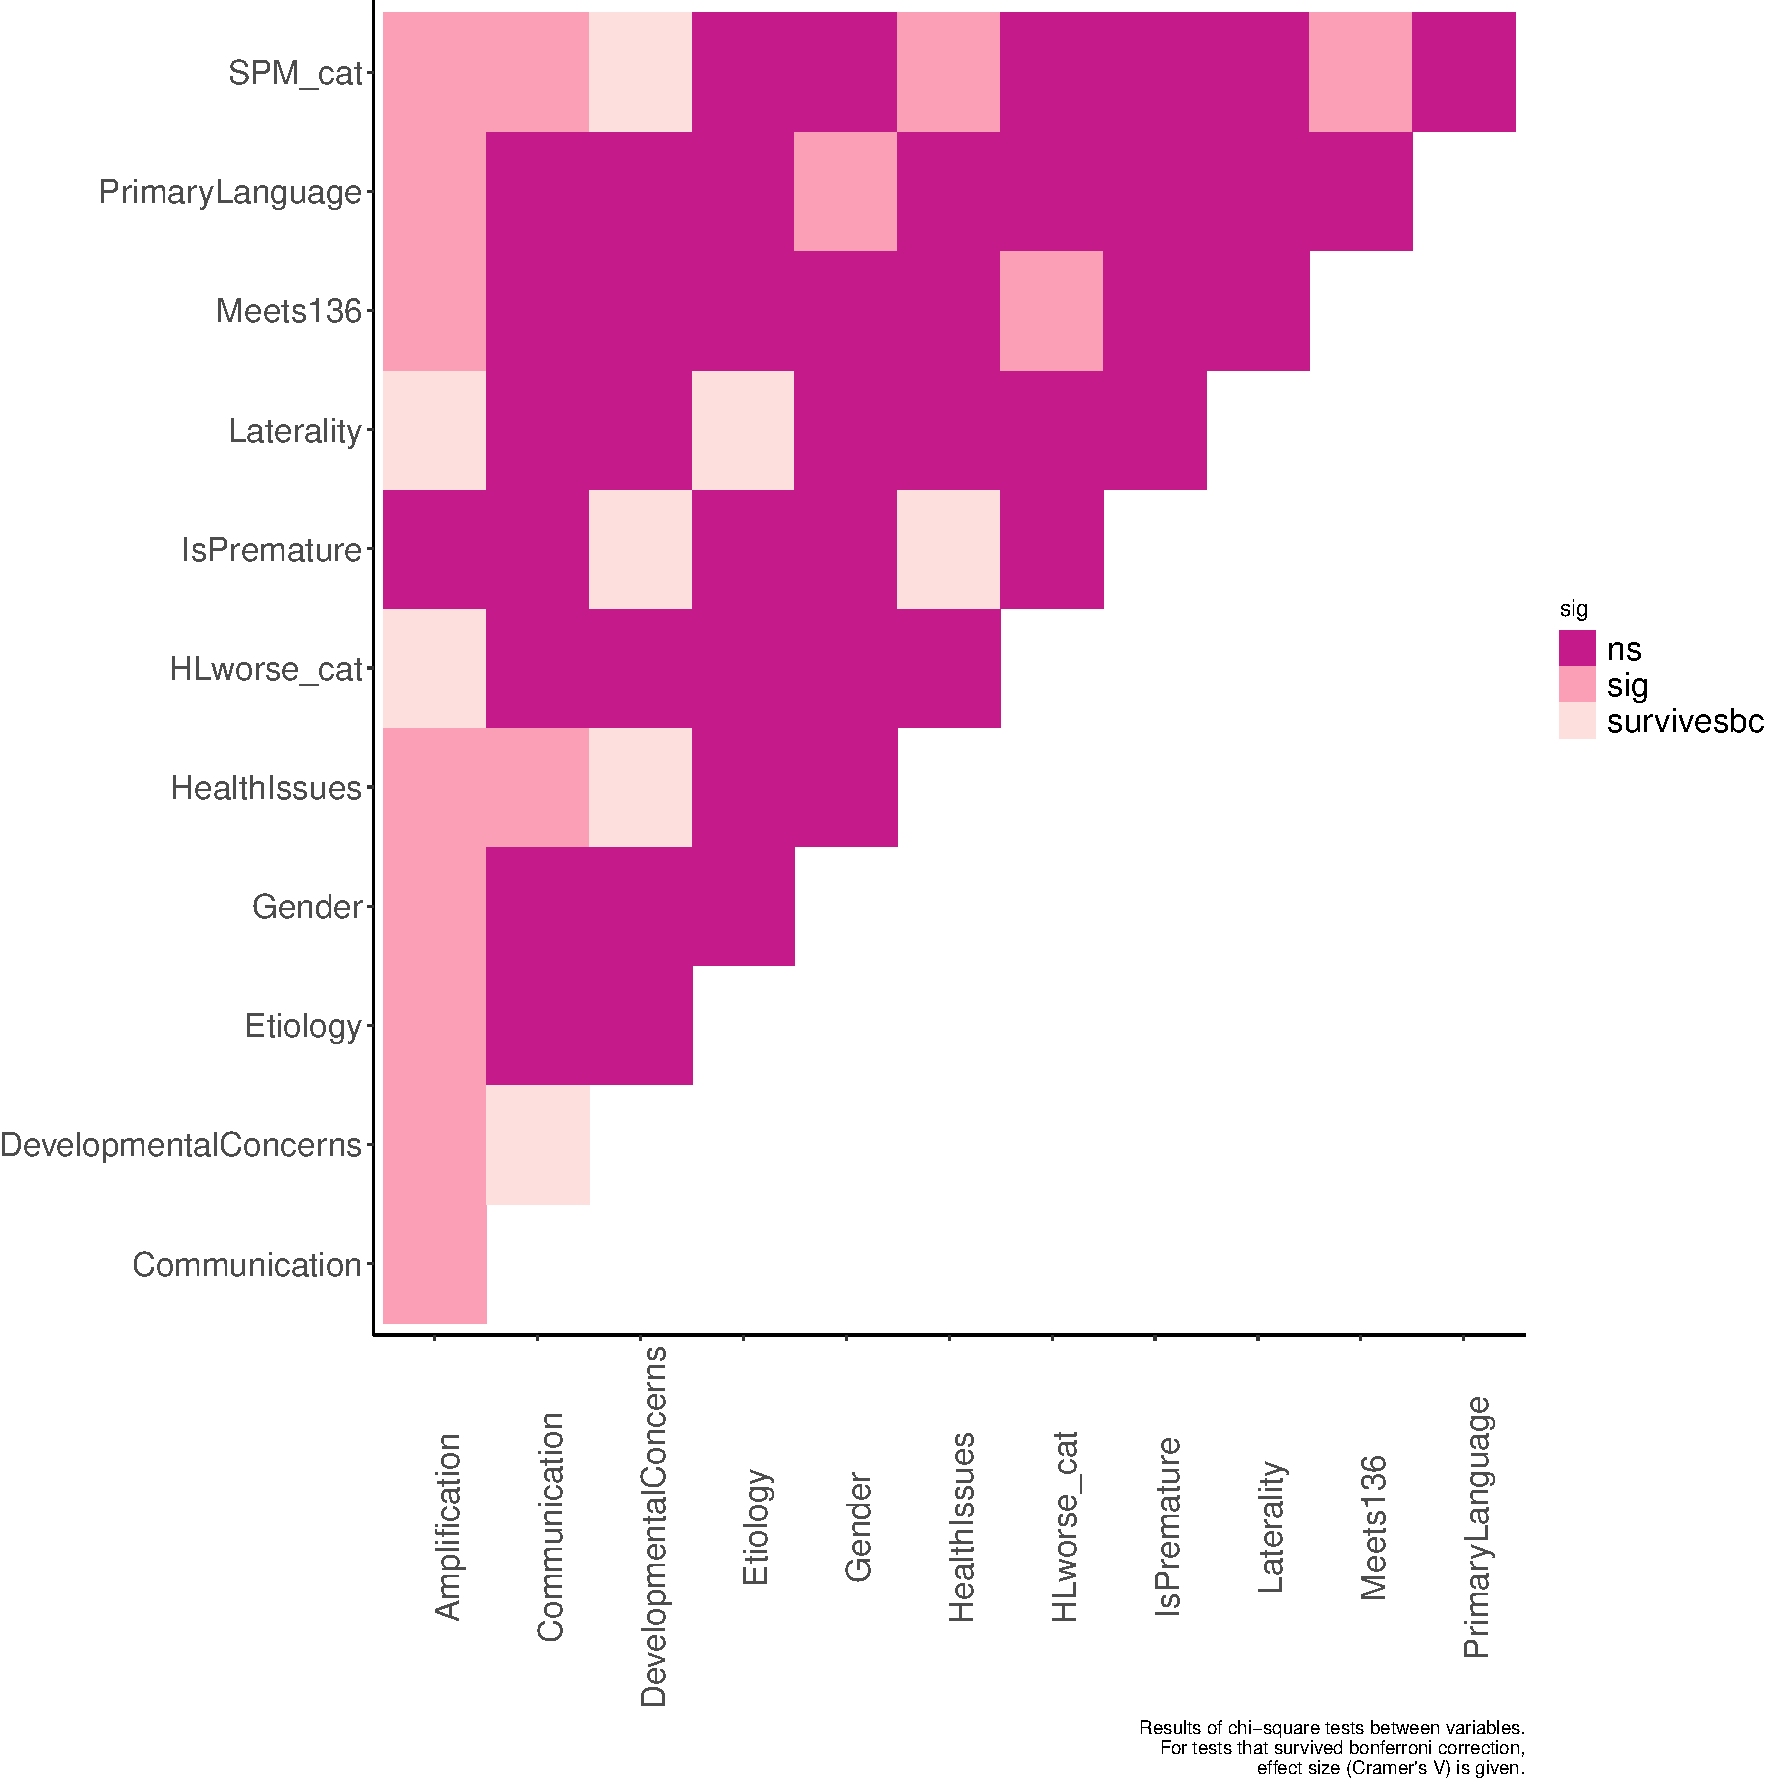
\includegraphics{ELSSP_paper_files/figure-latex/relationships-plot-1.pdf} 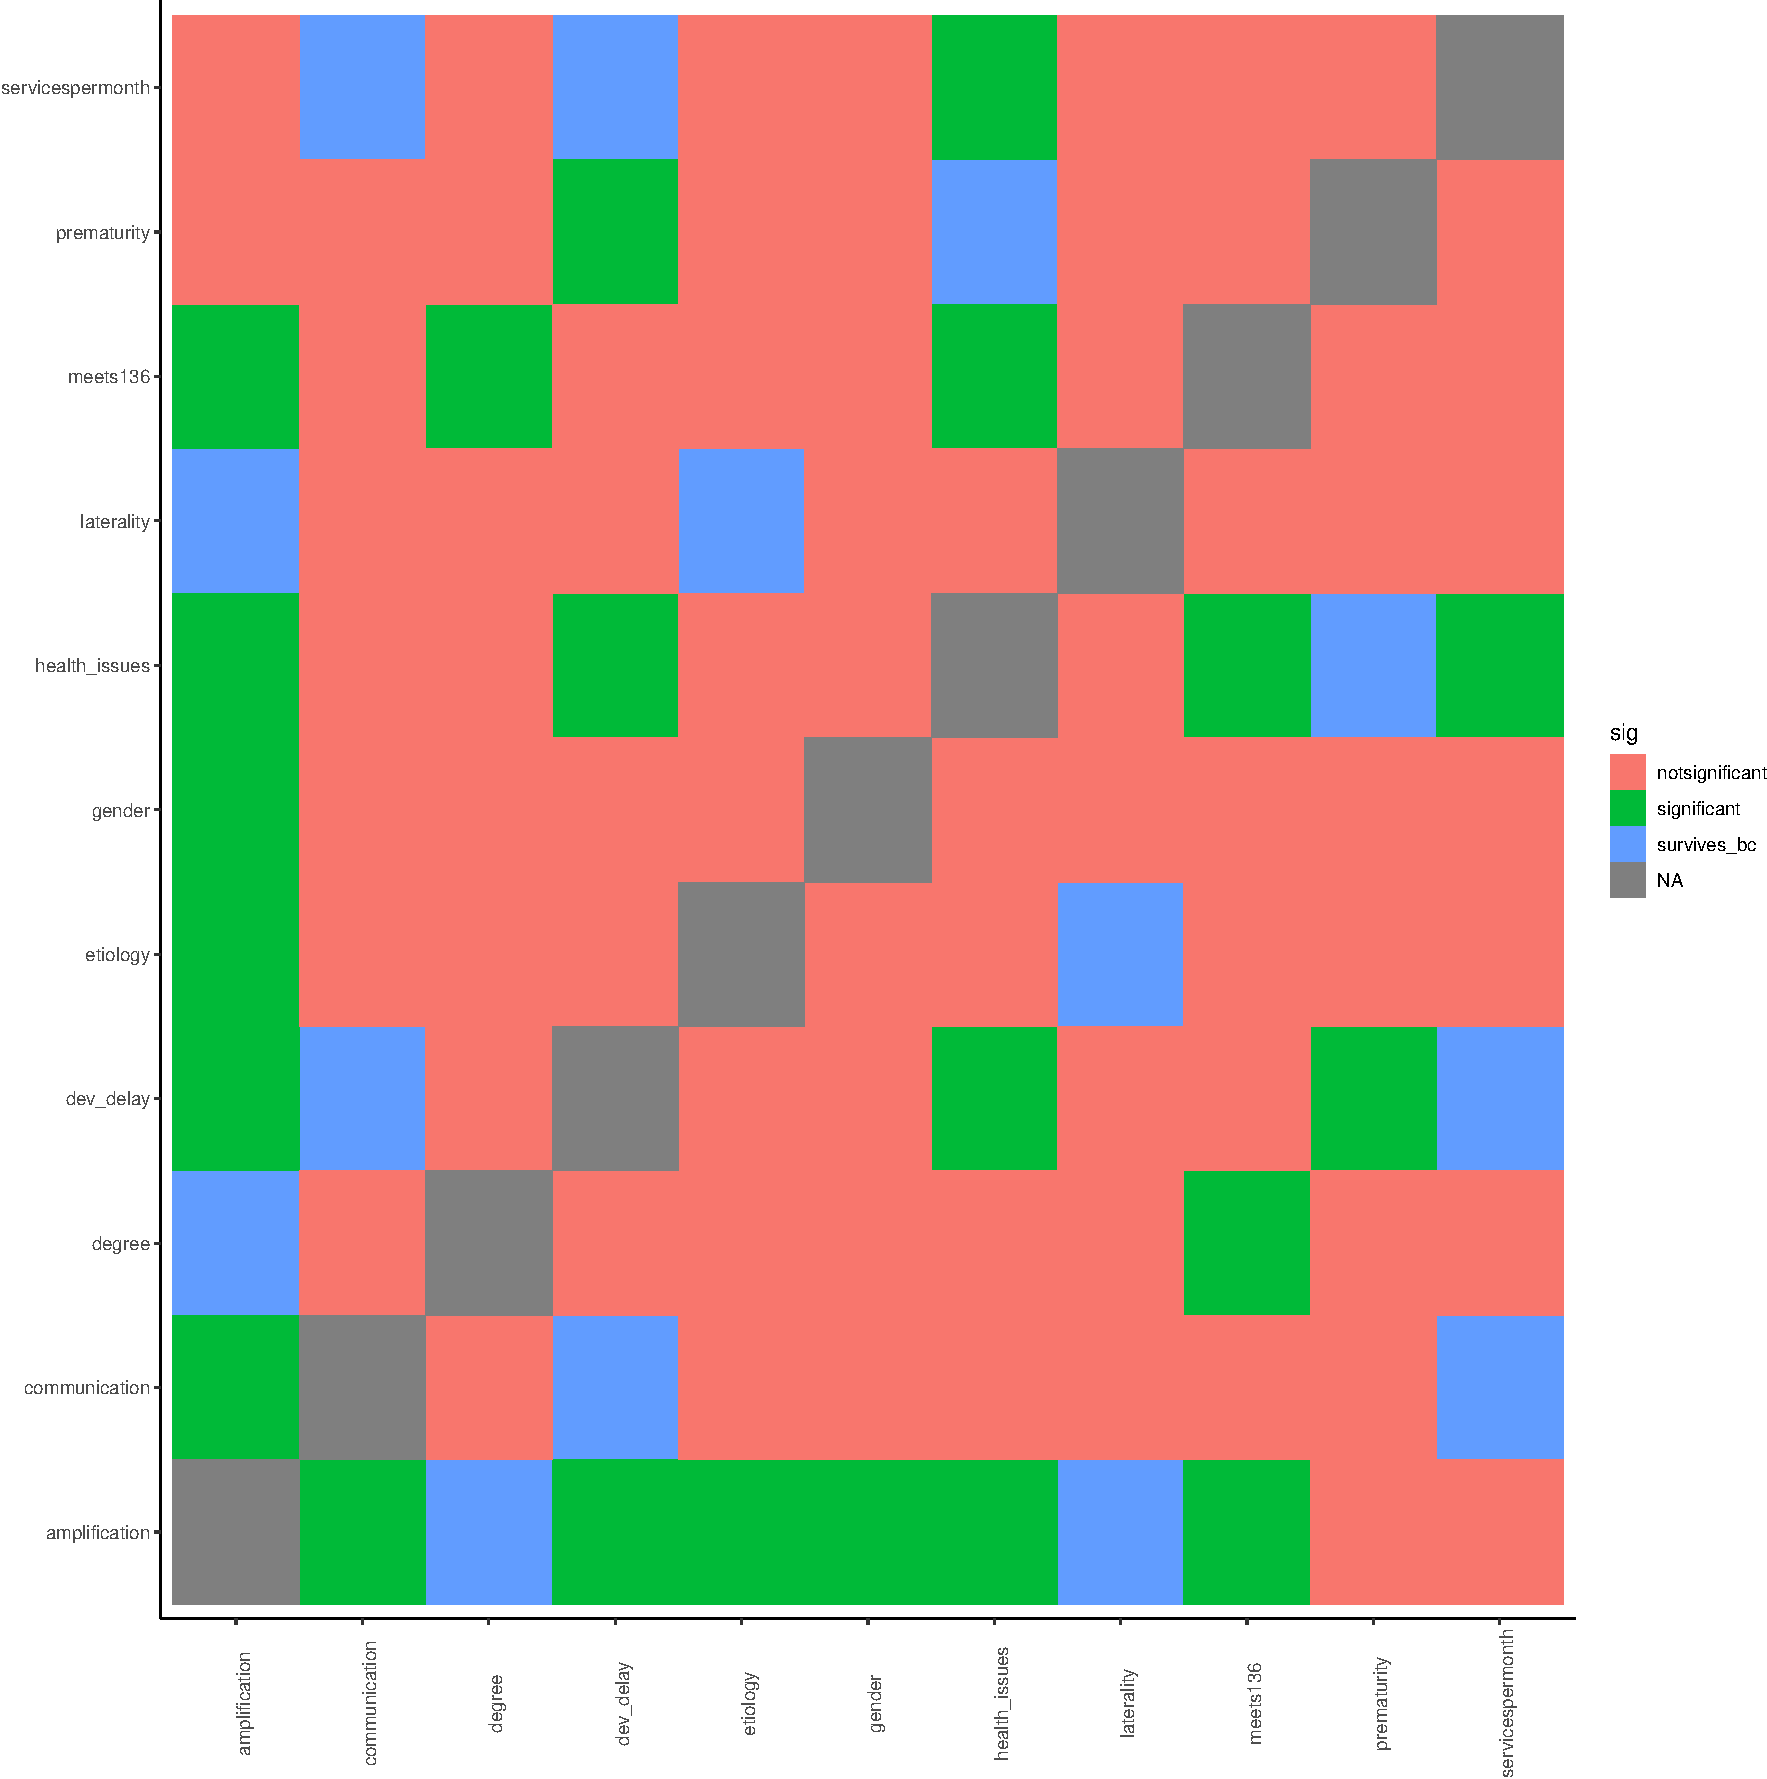
\includegraphics{ELSSP_paper_files/figure-latex/relationships-plot-2.pdf}

From this analysis, we found that children born premature were more likely to also have health issues (\(X^2\) (1, N = 96) = 25.69, p = 0). Children with conductive hearing loss were more likely to have unilateral hearing loss (\(X^2\) (2, N = 86) = 14.84, p = 6e-04). Children with unilateral hearing loss were unlikely to receive a cochlear implant and more likely to use no amplification (\(X^2\) (2, N = 96) = 17.19, p = 2e-04). Children with more severe hearing loss were more likely to use a cochlear implant than children with milder hearing loss (H(2)=23.80, p=0.00). Children with developmental delays received more services per month than typically developing DHH children (H()=134.50, p=0.00)and were more likely to use total communication (\(X^2\) (2, N = 96) = 19.38, p = 1e-04). Children who used total communication received more services per month than children using spoken language (H(1)=15.60, p=0.00).

\hypertarget{part-ii-influence-on-vocabulary}{%
\subsection{Part II: Influence on vocabulary}\label{part-ii-influence-on-vocabulary}}

We first constructed a binary logistic growth curve for vocabulary from the 50th percentile data for typically developing children from Wordbank. With this function, each participant's CDI score yielded a predicted age from the normative data. For each child, we subtracted this predicted age (given the score) from the child's actual age to give us a measure of delay in months. Descriptively, we found widespread vocabulary delays on both Words and Gestures and Words and Sentences, with the majority of DHH children testing around or below the 25th percentile for hearing children.

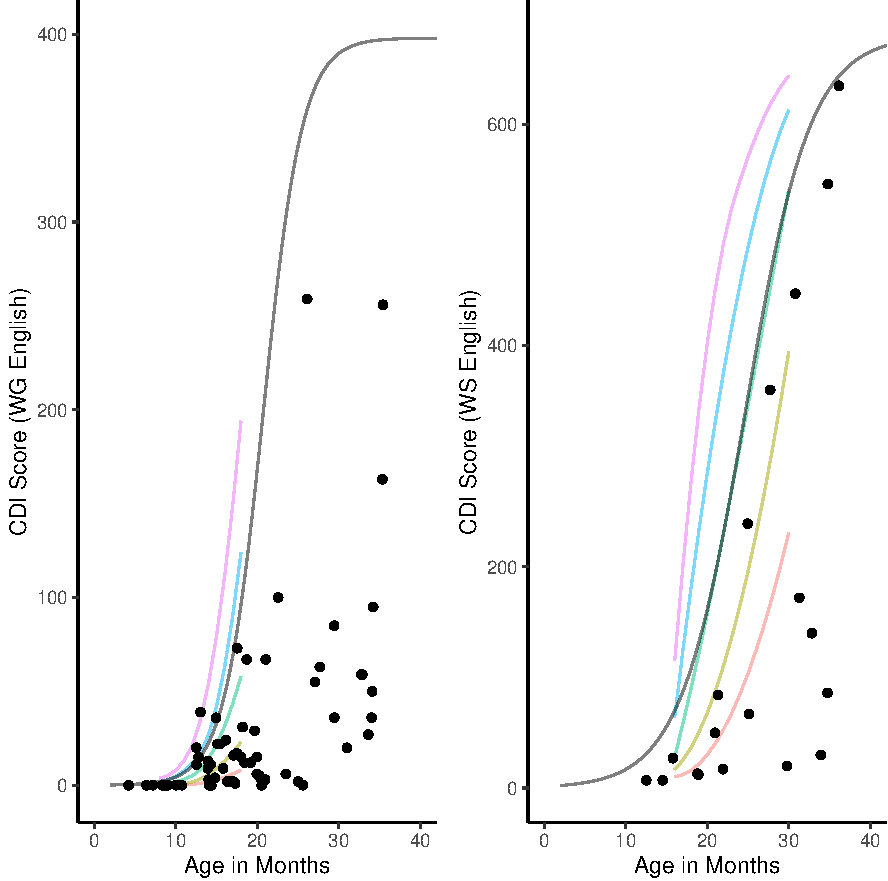
\includegraphics{ELSSP_paper_files/figure-latex/wg-ws-rainbow-plot-1.pdf}

We next explored the effect of the different audiological, demographic, and intervention characteristics on vocabulary delay. Vocabulary delay did not meet the assumption of normality, so we used non-parametric tests for the following set of analyses. Mann-Whitney-Wilcoxen tests were conducted to examine the effects of gender, laterality, developmental delay, health issues, prematurity, meeting 1-3-6 guidelines, and communication on vocabulary delay. We used kruskal-wallis tests for amplification and etiology, and Kendall's rank correlations for degree of hearing loss (worse ear) and services received per month. These results are exploratory and descriptive, and their interpretation should be tempered accordingly.

Boys were significantly more delayed than girls on Words and Sentences but not Words and Gestures. Children with developmental delays had larger vocabulary delays than children without developmental delays on Words and Gestures. Because only one child with a developmental delay took the Words and Sentences form, we did not perform the analysis for Words and Sentences. Premature children and children with health issues had smaller vocabularies than typically developing children on Words and Gestures but not Words and Sentences. Children who met 1-3-6 guidelines had larger vocabulary than children who did not on Words and Gestures but not Words and Sentences. On Words and Gestures but not Words and Sentences, receiving more early intervention services was correlated with lower vocabulary. We did not observe an effect of laterality, communication, degree, or etiology on vocabulary delay on either form of the CDI. For communication, we omitted cued speech from the analysis because only one child in our sample used this method of communication (shown on graph anyway for the curious). A kruskal-wallis test showed a significant effect of amplification on vocabulary delay on Words and Gestures, such that children with no amplification were more delayed than children without amplification.

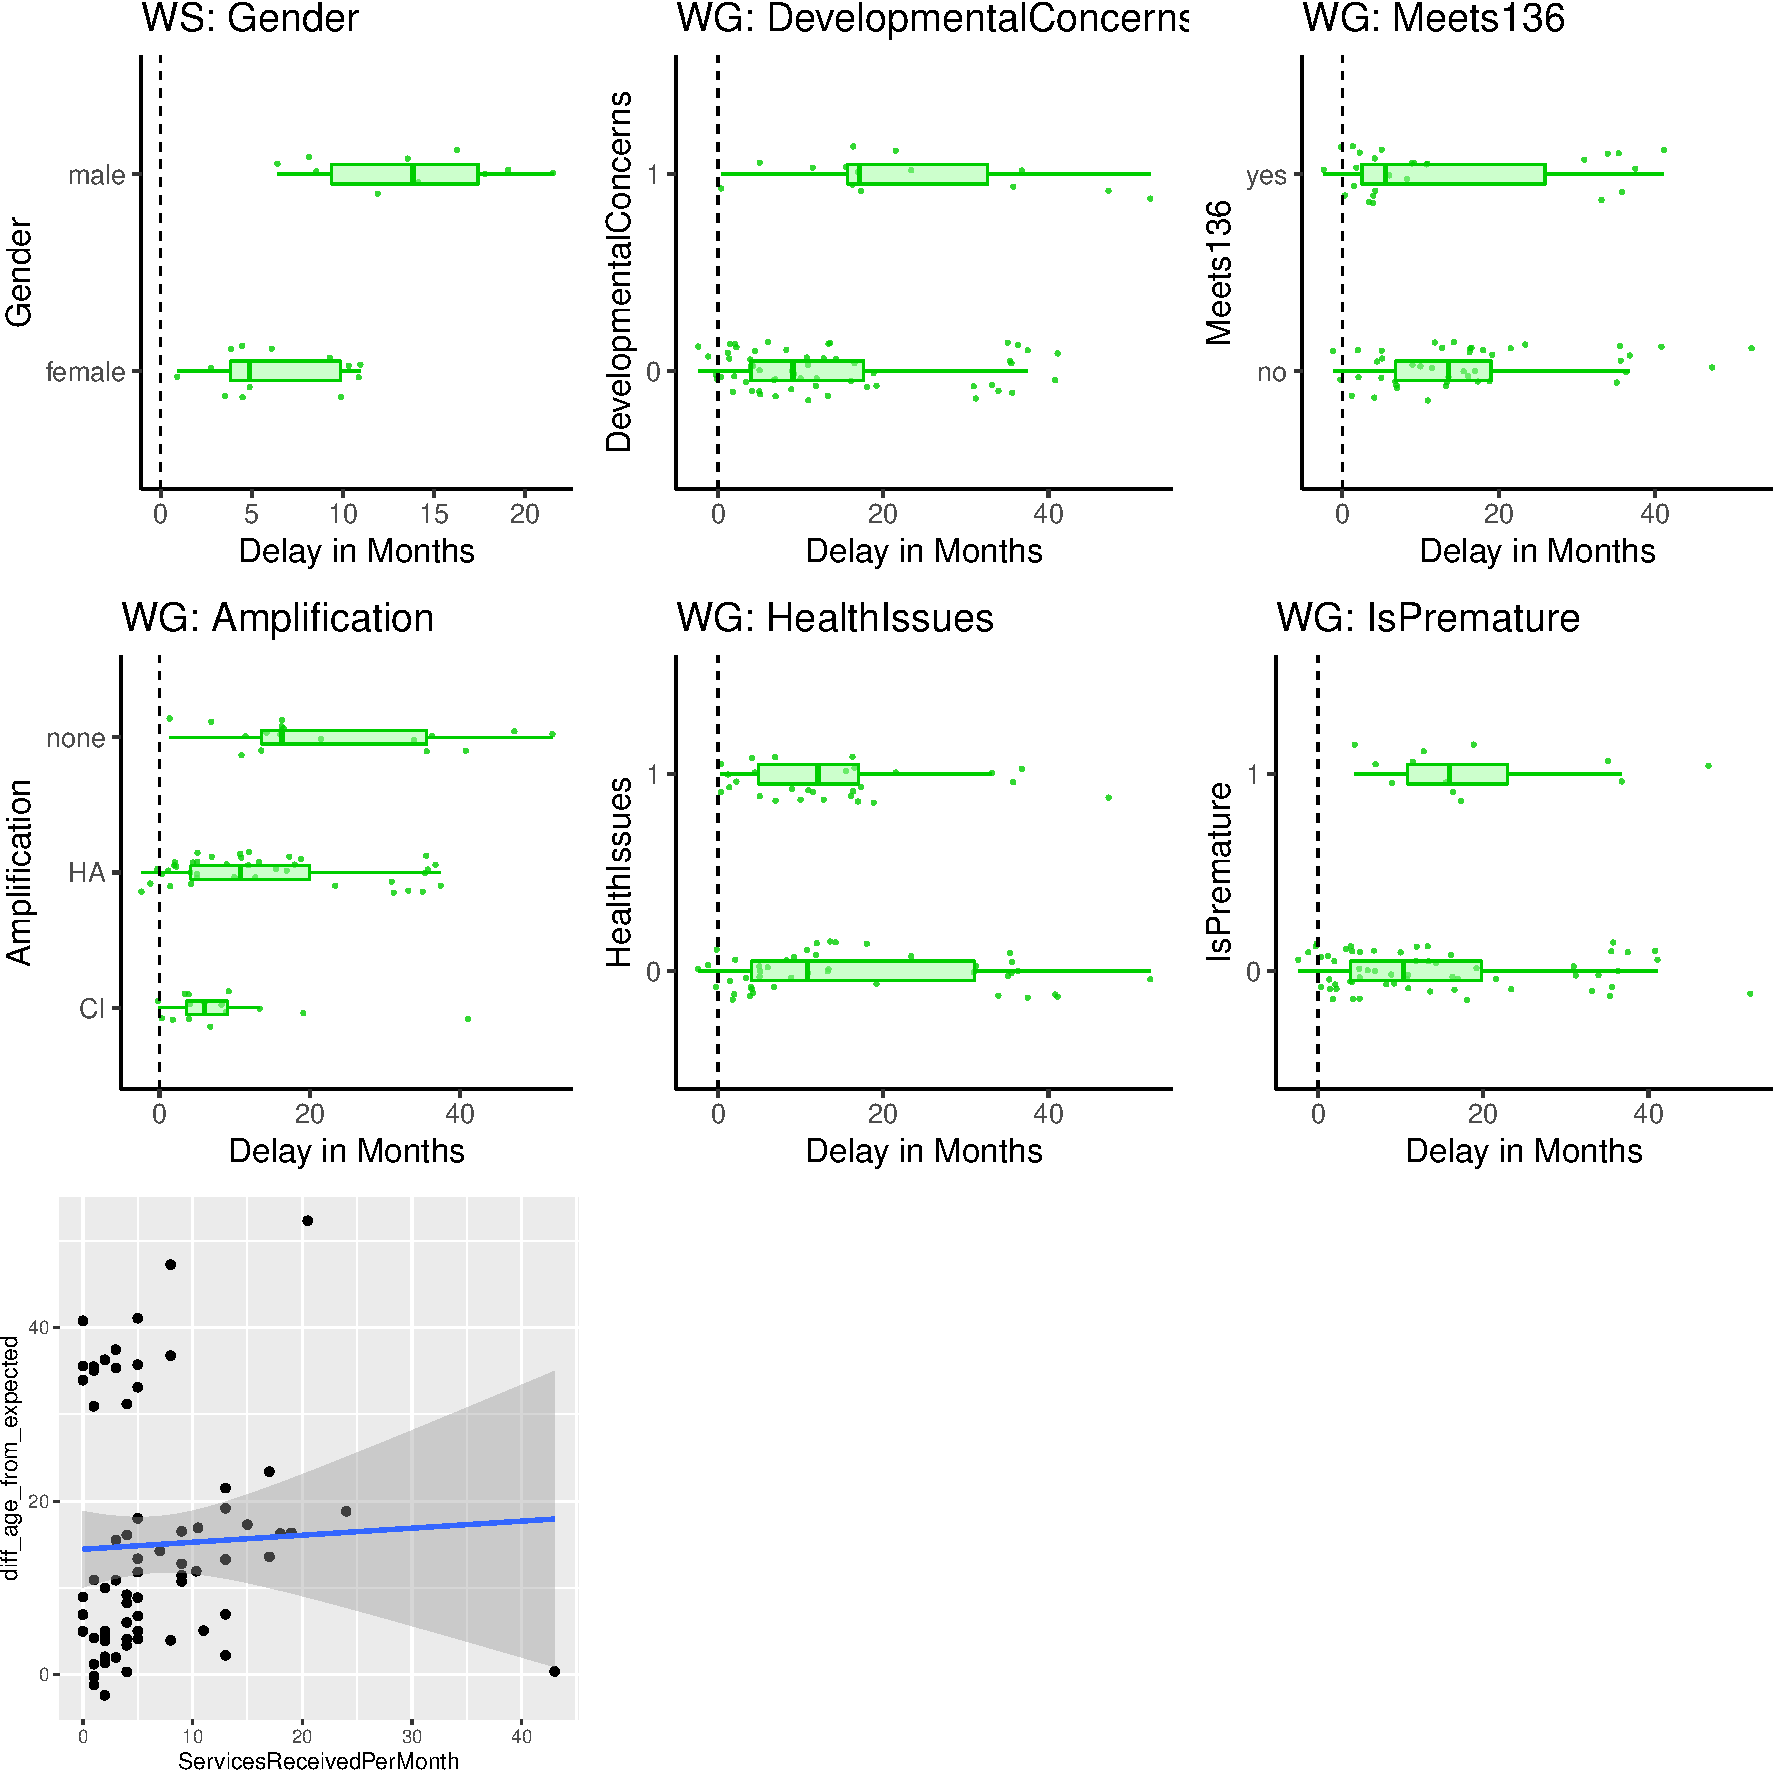
\includegraphics{ELSSP_paper_files/figure-latex/delay-plots-1.pdf}

\begin{table}

\caption{\label{tab:delay-table}Delay table}
\centering
\resizebox{\linewidth}{!}{
\begin{tabular}[t]{l|l|l|l}
\hline
Variable & WG mean delays & WS mean delays & Method\\
\hline
Gender & Boy: 17.4; Girl: 12 & Boy: 13.7; Girl: 6.3 & wilcox\\
\hline
Laterality & Unilateral: 13.3; Bilateral: 15.7 & Unilateral: 7.7; Bilateral: 11.1 & wilcox\\
\hline
Amplification & CI: 8.7; HA: 14.1, none: 23 & CI: 19.7; HA: 8.1, none: 10.3 & kruskall\\
\hline
Health Issues & Yes: 14.5; No: 15.5 & Yes: 8.2; No: 10.3 & wilcox\\
\hline
Developmental Delay & Yes: 23.9; No: 13.1 & Yes: 4.5; No: 10.1 & wilcox\\
\hline
Prematurity & Premature: 19.3; Full-term: 14.3 & Premature: 8.9; Full-term: 10 & wilcox\\
\hline
1-3-6 Guidelines & Meets: 12.7; Does not meet: 16.6 & Meets: 10.8; Does not meet: 9.4 & wilcox\\
\hline
Communication & Spoken Language: 13.8; Total Communication: 21.2 & Spoken Language: 10.2; Total Communication: 6 & wilcox\\
\hline
Etiology & SNHL: 14.5; Mixed: 18.8, Conductive: 16.4 & SNHL: 8.5; Mixed: 15.8, Conductive: 8 & kruskall\\
\hline
Degree & More severe: 15.2; Less severe: 15.2 & More severe: 10.8; Less severe: 9.5 & wilcox\\
\hline
Services Received Per Month & More services: 17.6; Less services: 13.7 & More services: 12.5; Less services: 9.1 & wilcox\\
\hline
\end{tabular}}
\end{table}

\hypertarget{part-iii-meets136-success}{%
\subsection{Part III: Meets136 success}\label{part-iii-meets136-success}}

Lastly, we looked at the ages at which children received diagnosis and intervention, and how this mapped onto the 1-3-6 guidelines. 36.84\% of our sample met 1-3-6 guidelines for early diagnosis and intervention. Of children with comorbidities (i.e., developmental concerns, prematurity, health issues, vision loss), only 22\% met 1-3-6 guidelines, compared to 45.76\% of typically developing children.

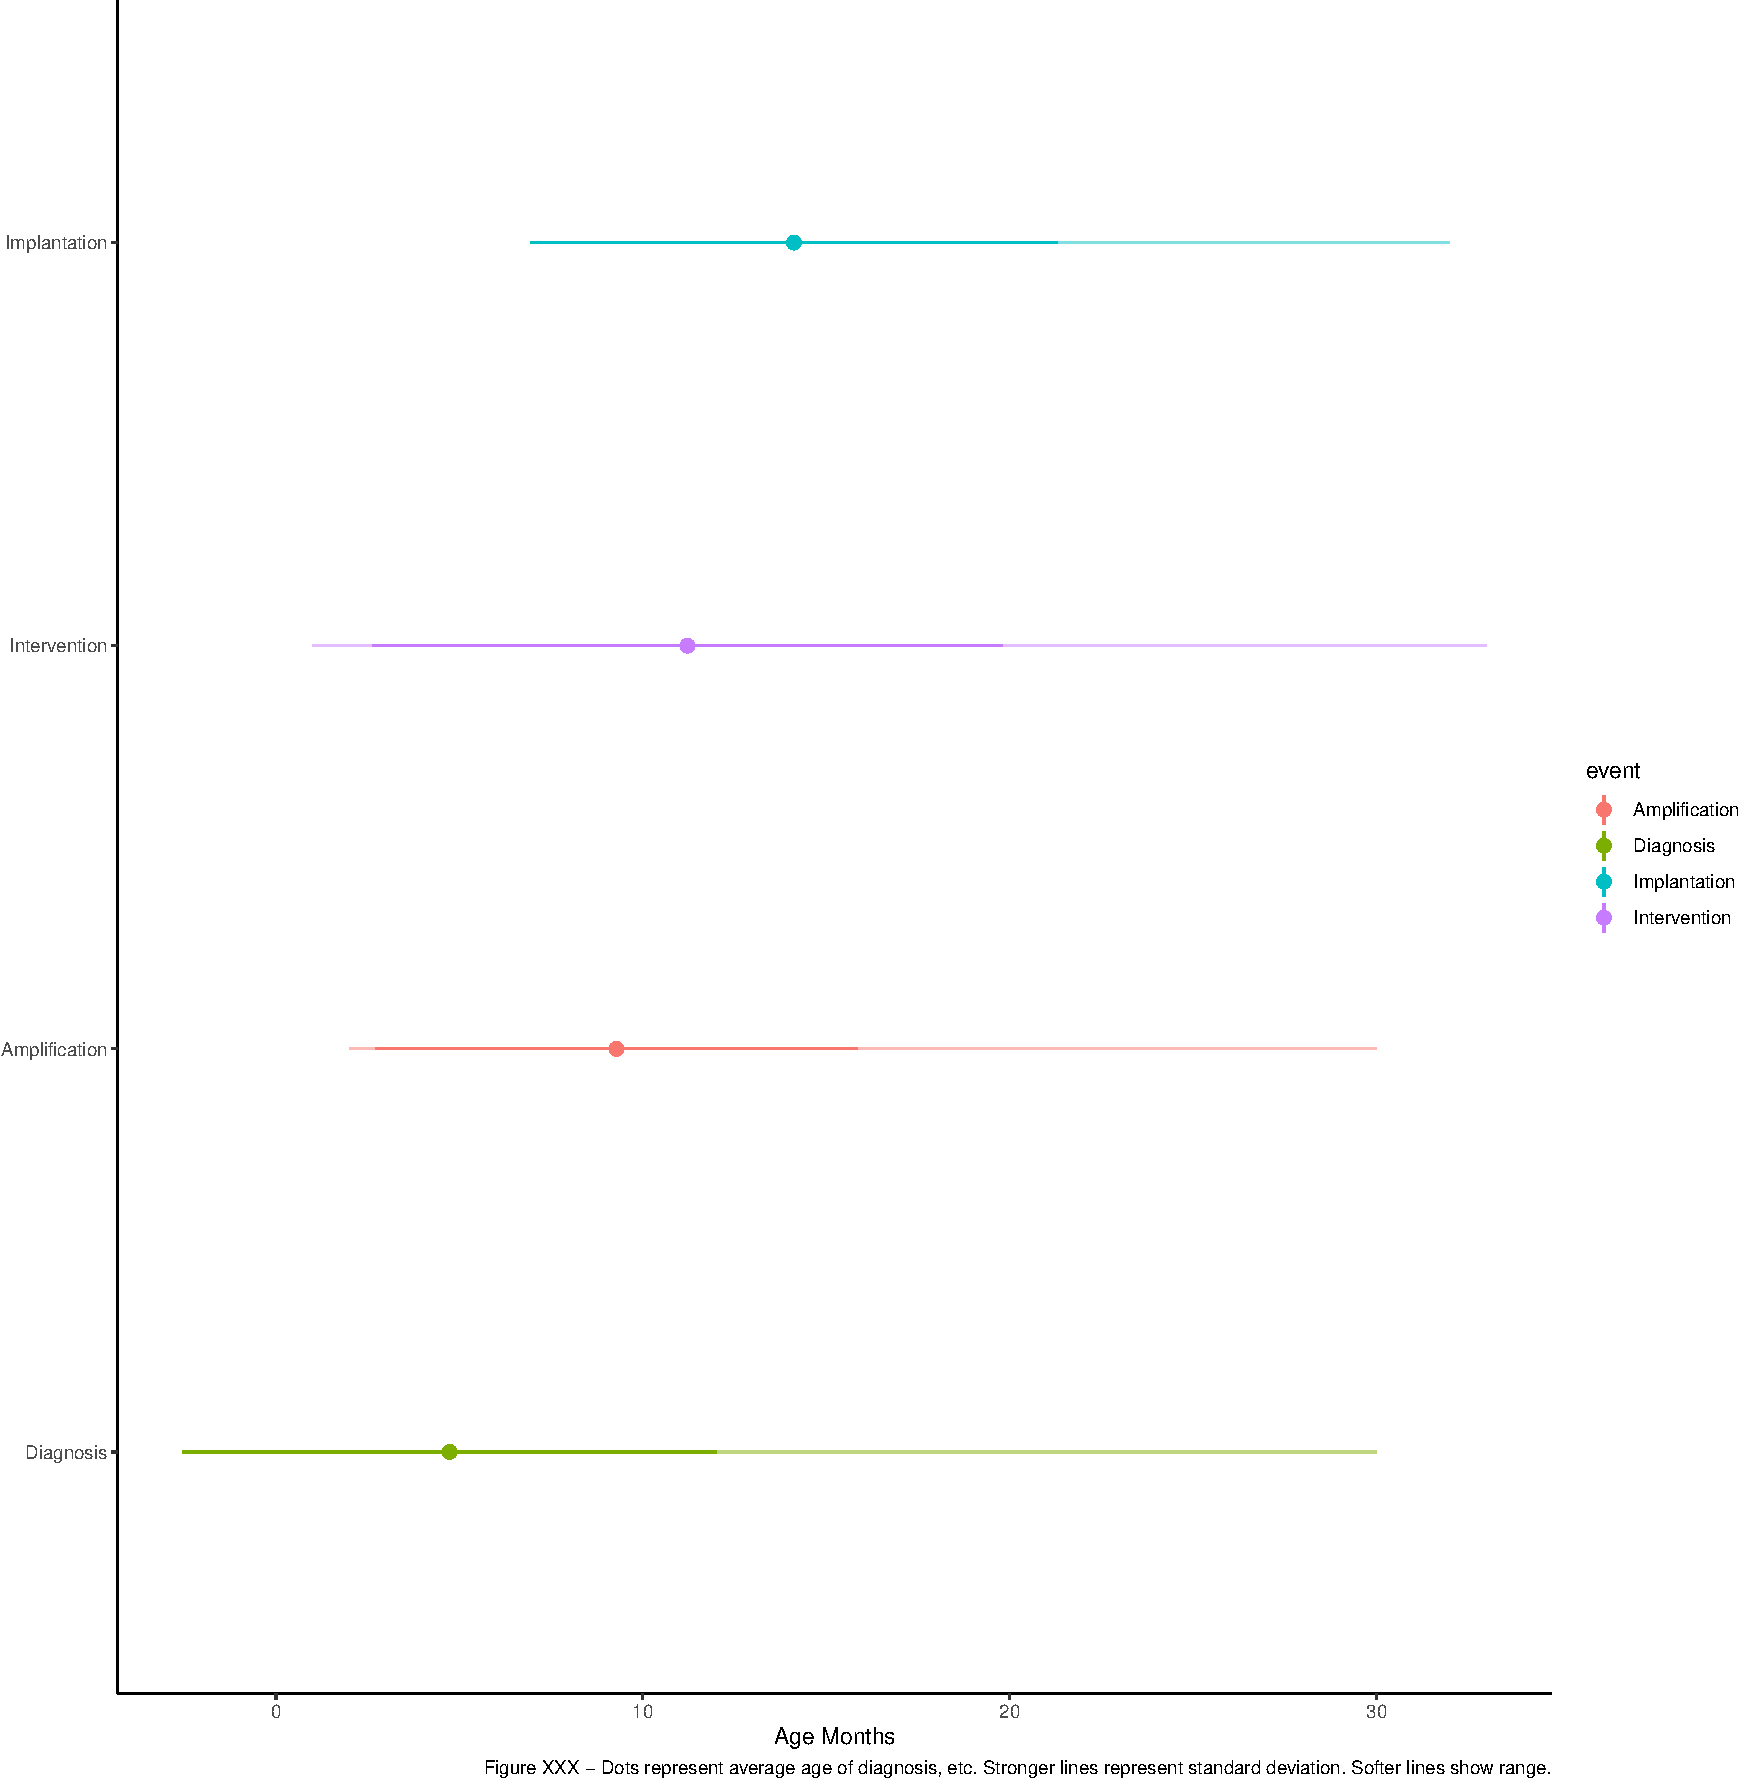
\includegraphics{ELSSP_paper_files/figure-latex/meets136-timeline-1.pdf}

We created linear regression models for age at diagnosis and age at intervention. Models were paired down using stepwise regression by AIC using the stepAIC function (cite MASS package). For age at diagnosis, we included the set of child-specific factors that would be relevant before diagnosis of hearing loss. We began with:
Age diagnosis \textasciitilde{} gender + laterality + degree (worse ear) + developmental delay + health issues + prematurity + laterality + language background + etiology
The best fit model (R2=0.19 , p=0.00 )included health issues (\(eta\) = 3.96, p = 0.00676700971366628) and language background (\(eta\) = -7.04, p = 0.000604603179891035).
Age diagnosis \textasciitilde{} health issues + language background

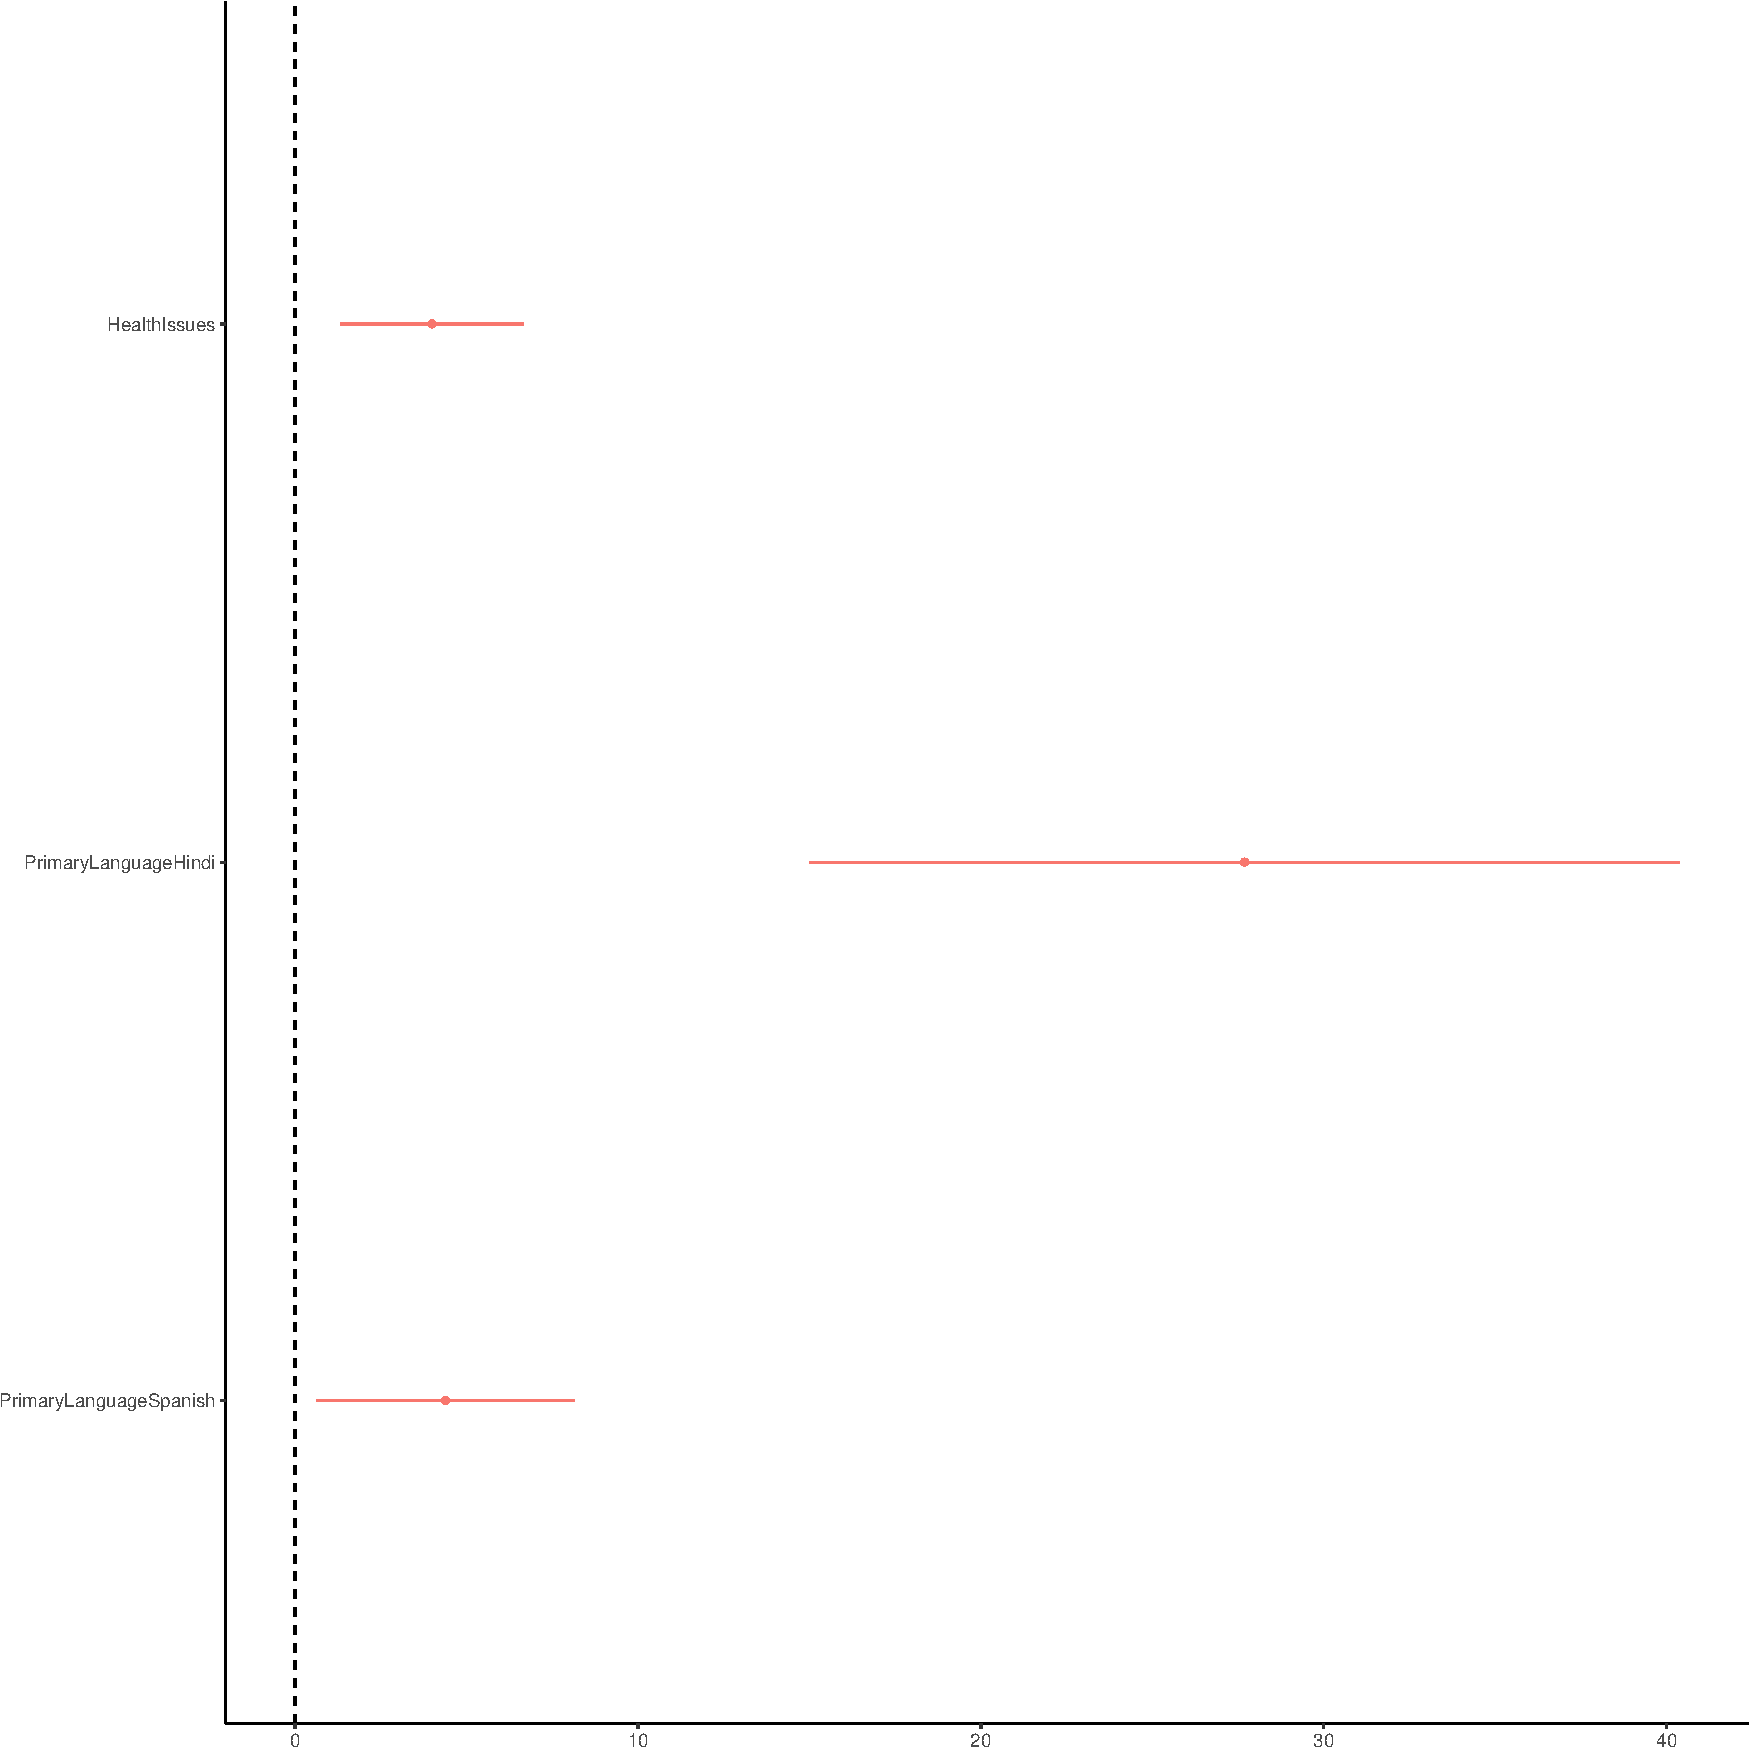
\includegraphics{ELSSP_paper_files/figure-latex/diagnosis-betas-1.pdf}

For age at intervention, we first included the variables potentially relevant prior to intervention:
Age intervention \textasciitilde{} gender + degree (worse ear) + developmental delay + health issues + prematurity + laterality + language background + etiology + age diagnosis
The best fit model (R2=0.41 , p=0.00) included prematurity (\(eta\) = 4.05, p = 0.0582176683126837), laterality (\(eta\) = -2.44, p = 0.194119668422873), degree of hearing loss (\(eta\) = -0.09, p = 0.00910803624304661), and age at diagnosis (\(eta\) = 0.62, p = 9.38566161533036e-08).
Age intervention \textasciitilde{} laterality + degree (worse ear) + prematurity + laterality + age diagnosis

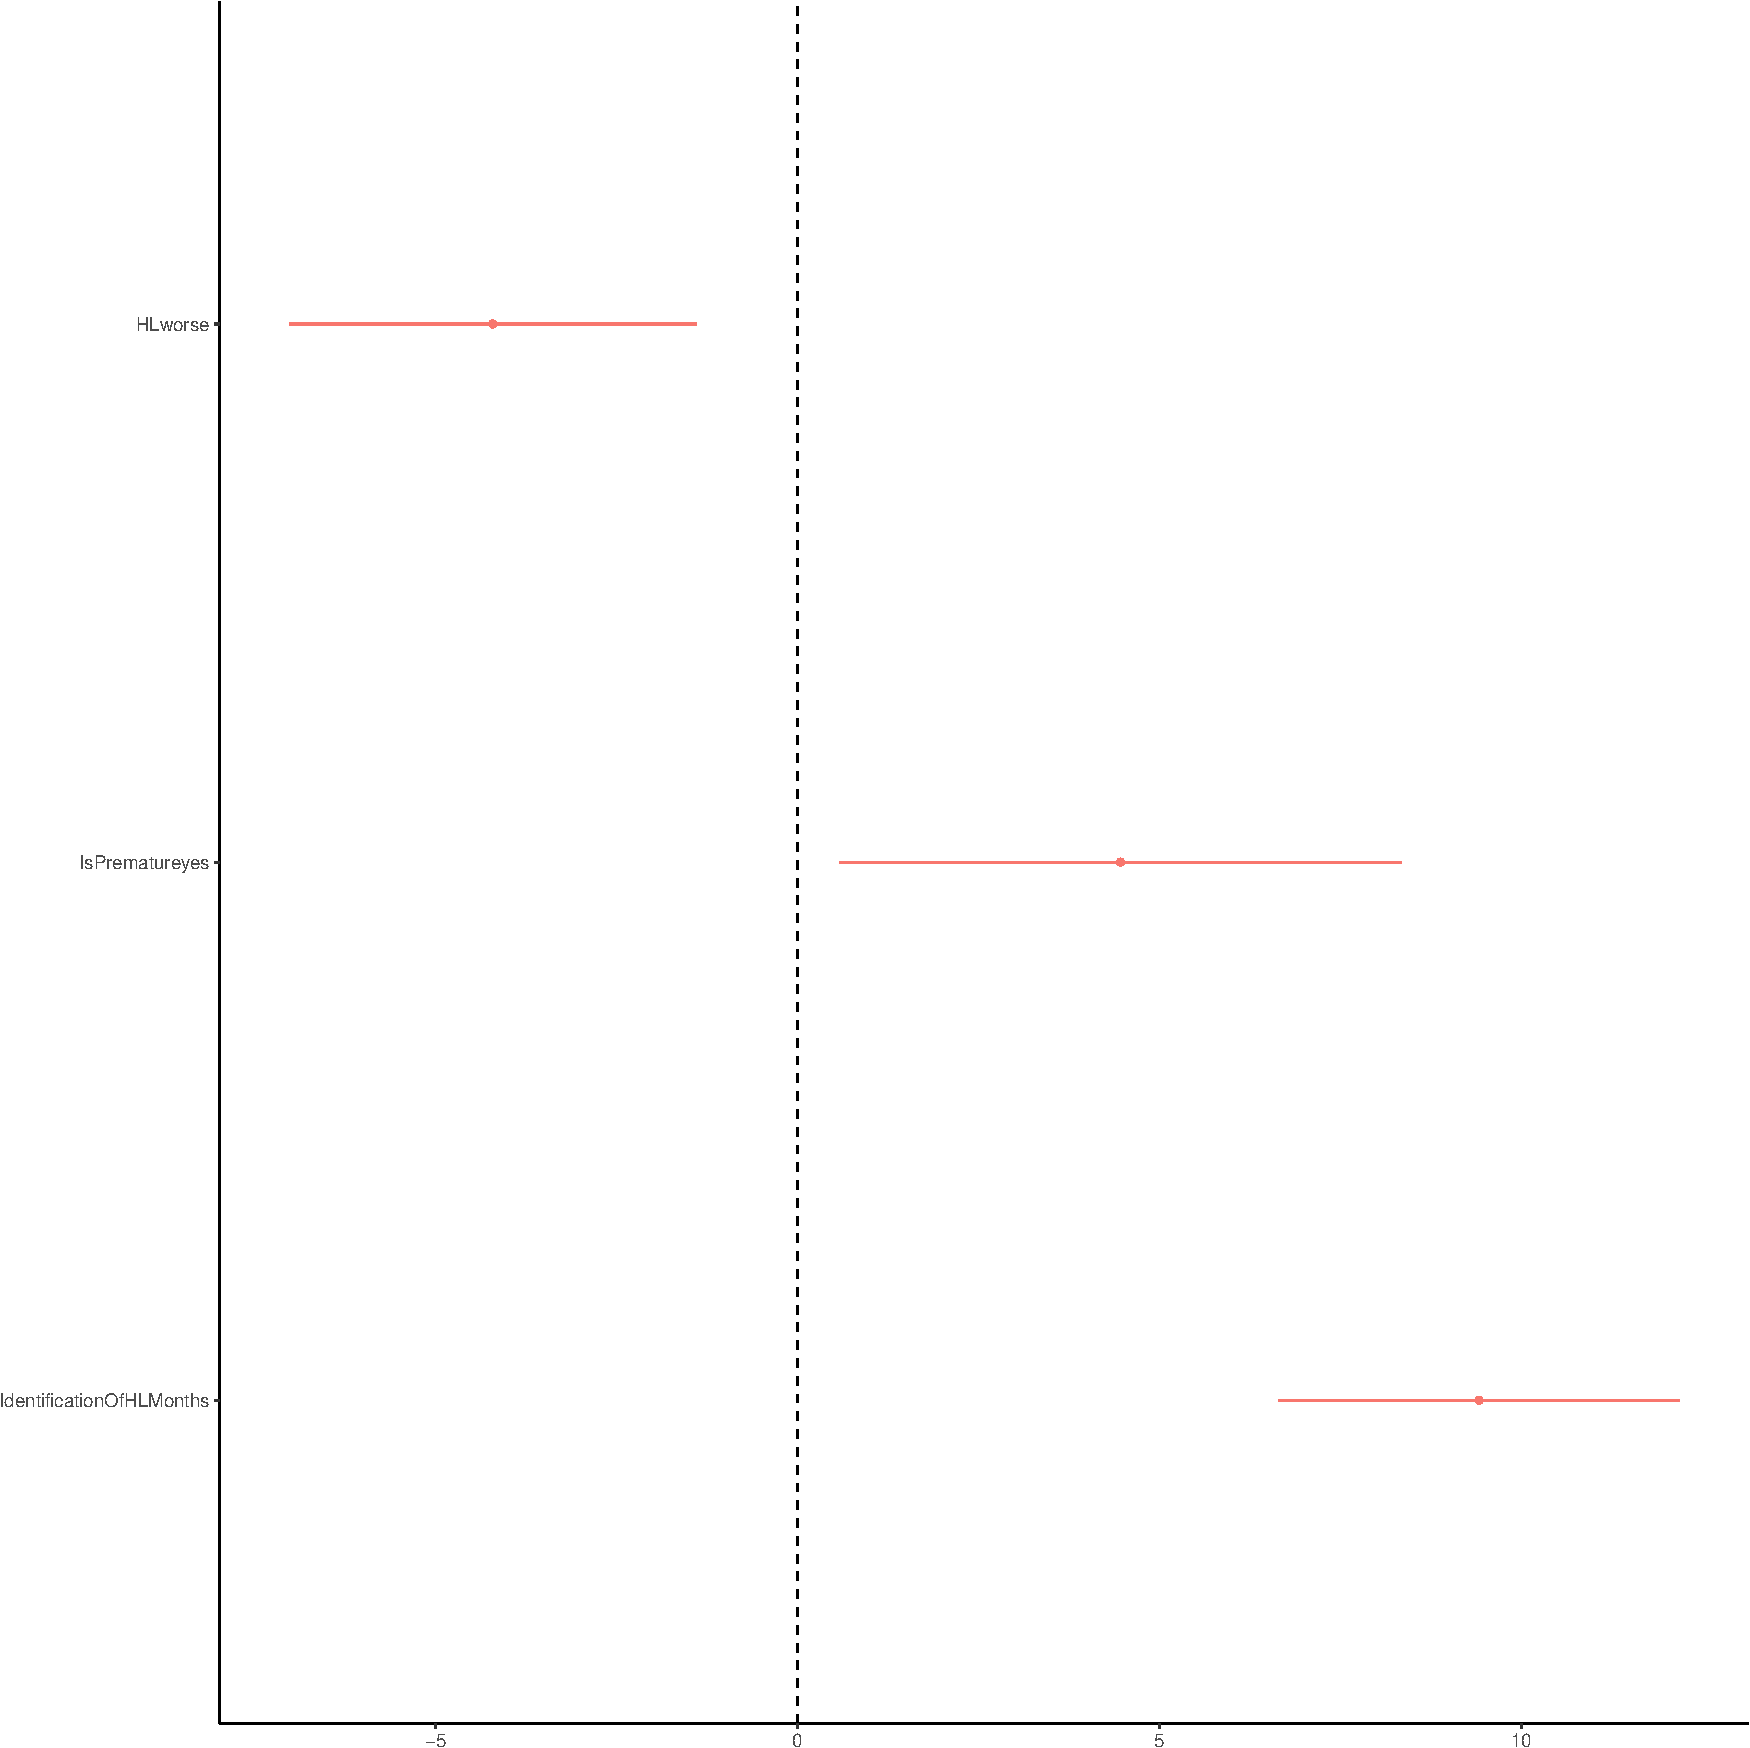
\includegraphics{ELSSP_paper_files/figure-latex/intervention-betas-1.pdf}
\# Discussion

\hypertarget{conclusion}{%
\section{Conclusion}\label{conclusion}}

Footnotes: Despite exciting, increasing, and converging evidence for benefits of early sign language exposure (e.g., Schick, De Villiers, De Villiers, \& Hoffmeister, 2007; Clark et al., 2016; Davidson, Lillo-Martin, \& Pichler, 2014; Hrastinski \& Wilbur, 2016; Magnuson, 2000; Spencer, 1993), the majority of DHH children will not be raised in a sign language environment. This is particularly true for North Carolina, which does not have a large community of sign language users, relative to states like Maryland or areas like Washington D.C. or Rochester, NY. For this reason, we focus on spoken language development.

\hypertarget{references}{%
\section*{References}\label{references}}
\addcontentsline{toc}{section}{References}

\hypertarget{refs}{}
\leavevmode\hypertarget{ref-2000}{}%
15A NCAC 21F .1201 - .1204. (2000).

\leavevmode\hypertarget{ref-amin2014}{}%
Amin, S. B., Vogler-Elias, D., Orlando, M., \& Wang, H. (2014). Auditory neural myelination is associated with early childhood language development in premature infants. \emph{Early Human Development}, \emph{90}(10), 673--678. \url{https://doi.org/10.1016/j.earlhumdev.2014.07.014}

\leavevmode\hypertarget{ref-anderson2002}{}%
Anderson, D., \& Reilly, J. (2002). The MacArthur Communicative Development Inventory: Normative Data for American Sign Language. \emph{Journal of Deaf Studies and Deaf Education}, \emph{7}(2), 83--106. \url{https://doi.org/10.1093/deafed/7.2.83}

\leavevmode\hypertarget{ref-anne2017}{}%
Anne, S., Lieu, J. E. C., \& Cohen, M. S. (2017). Speech and Language Consequences of Unilateral Hearing Loss: A Systematic Review. \emph{Otolaryngologyhead and Neck Surgery : Official Journal of American Academy of Otolaryngology-Head and Neck Surgery}, \emph{157}(4), 572--579. \url{https://doi.org/10.1177/0194599817726326}

\leavevmode\hypertarget{ref-apuzzo1995}{}%
Apuzzo, M.-R. L., \& Yoshinaga-Itano, C. (1995). \emph{Early Identification of Infants with Significant Hearing Loss and the Minnesota Child Development Inventory} (No. 2). \emph{SEMINARS IN HEARING-VOLUME} (Vol. 16).

\leavevmode\hypertarget{ref-artieres2009}{}%
Artières, F., Vieu, A., Mondain, M., Uziel, A., \& Venail, F. (2009). Impact of early cochlear implantation on the linguistic development of the deaf child. \emph{Otology and Neurotology}, \emph{30}(6), 736--742. \url{https://doi.org/10.1097/MAO.0b013e3181b2367b}

\leavevmode\hypertarget{ref-barre2011}{}%
Barre, N., Morgan, A., Doyle, L. W., \& Anderson, P. J. (2011). Language abilities in children who were very preterm and/or very low birth weight: A meta-analysis. \emph{Journal of Pediatrics}, \emph{158}(5). \url{https://doi.org/10.1016/j.jpeds.2010.10.032}

\leavevmode\hypertarget{ref-birman2012}{}%
Birman, C. S., Elliott, E. J., \& Gibson, W. P. (2012). Pediatric cochlear implants: Additional disabilities prevalence, risk factors, and effect on language outcomes. \emph{Otology and Neurotology}, \emph{33}(8), 1347--1352. \url{https://doi.org/10.1097/MAO.0b013e31826939cc}

\leavevmode\hypertarget{ref-blair1985}{}%
Blair, J. C., Peterson, M., \& Viehweg, S. (1985). The Effects of Mild Sensorineural Hearing Loss on Academic Performance of Young School-Age Children. \emph{Volta Review}, \emph{87}(2), 87--93.

\leavevmode\hypertarget{ref-bornstein2004}{}%
Bornstein, M. H., Hahn, C.-S., \& Haynes, O. M. (2004). Specific and general language performance across early childhood: Stability and gender considerations. \emph{First Language}, \emph{24}(3), 267--304. \url{https://doi.org/10.1177/0142723704045681}

\leavevmode\hypertarget{ref-branson2009}{}%
Branson, D., \& Demchak, M. (2009). The Use of Augmentative and Alternative Communication Methods with Infants and Toddlers with Disabilities: A Research Review. \emph{Augmentative and Alternative Communication}, \emph{25}(4), 274--286. \url{https://doi.org/10.3109/07434610903384529}

\leavevmode\hypertarget{ref-bruce2015}{}%
Bruce, S. M., \& Borders, C. (2015). Communication and Language in Learners Who Are Deaf and Hard of Hearing With Disabilities: Theories, Research, and Practice. \emph{American Annals of the Deaf}, \emph{160}(4), 368--384. \url{https://doi.org/10.1353/aad.2015.0035}

\leavevmode\hypertarget{ref-capps2009}{}%
Capps, L. (2009). H.R.1246 - 111th Congress (2009-2010): Early Hearing Detection and Intervention Act of 2009.

\leavevmode\hypertarget{ref-carter2017}{}%
Carter, F. A., \& Msall, M. E. (2017). \emph{Language Abilities as a Framework for Understanding Emerging Cognition and Social Competencies after Late, Moderate, and Very Preterm Birth}. \emph{Journal of Pediatrics} (Vol. 181). Mosby Inc. \url{https://doi.org/10.1016/j.jpeds.2016.10.077}

\leavevmode\hypertarget{ref-castellanos2016}{}%
Castellanos, I., Pisoni, D. B., Kronenberger, W. G., \& Beer, J. (2016). Early expressive language skills predict long-term neurocognitive outcomes in cochlear implant users: Evidence from the MacArthurBates Communicative Development Inventories. \emph{American Journal of Speech-Language Pathology}, \emph{25}(3), 381--392. \url{https://doi.org/10.1044/2016_AJSLP-15-0023}

\leavevmode\hypertarget{ref-cdc2018}{}%
CDC. (2018). 2016 Hearing Screening Summary. \emph{Centers for Disease Control and Prevention}. https://www.cdc.gov/ncbddd/hearingloss/2016-data/01-data-summary.html.

\leavevmode\hypertarget{ref-chapman1997}{}%
Chapman, R. S. (1997). Language development in children and adolescents with Down syndrome. \emph{Mental Retardation and Developmental Disabilities Research Reviews}, \emph{3}(4), 307--312. \href{https://doi.org/10.1002/(SICI)1098-2779(1997)3:4\%3C307::AID-MRDD5\%3E3.0.CO;2-K}{https://doi.org/10.1002/(SICI)1098-2779(1997)3:4\textless{}307::AID-MRDD5\textgreater{}3.0.CO;2-K}

\leavevmode\hypertarget{ref-ching2010}{}%
Ching, T. Y., Crowe, K., Martin, V., Day, J., Mahler, N., Youn, S., \ldots{} Orsini, J. (2010). Language development and everyday functioning of children with hearing loss assessed at 3 years of age. In \emph{International Journal of Speech-Language Pathology} (Vol. 12, pp. 124--131). \url{https://doi.org/10.3109/17549500903577022}

\leavevmode\hypertarget{ref-ching2013}{}%
Ching, T. Y., Dillon, H., Marnane, V., Hou, S., Day, J., Seeto, M., \ldots{} Yeh, A. (2013). Outcomes of early- and late-identified children at 3 years of age: Findings from a prospective population-based study. \emph{Ear and Hearing}, \emph{34}(5), 535--552. \url{https://doi.org/10.1097/AUD.0b013e3182857718}

\leavevmode\hypertarget{ref-ching2007}{}%
Ching, T. Y., Van Wanrooy, E., \& Dillon, H. (2007). \emph{Binaural-Bimodal Fitting or Bilateral Implantation for Managing Severe to Profound Deafness: A Review}. \emph{Trends in Amplification} (Vol. 11). \url{https://doi.org/10.1177/1084713807304357}

\leavevmode\hypertarget{ref-clark1981}{}%
Clark, J. G. (1981). Uses and abuses of hearing loss classification. \emph{ASHA: A Journal of the American Speech-Language-Hearing Association}, \emph{23}(7), 493--500.

\leavevmode\hypertarget{ref-clark2016}{}%
Clark, M. D., Hauser, P. C., Miller, P., Kargin, T., Rathmann, C., Guldenoglu, B., \ldots{} Israel, E. (2016). The Importance of Early Sign Language Acquisition for Deaf Readers. \emph{Reading and Writing Quarterly}, \emph{32}(2), 127--151. \url{https://doi.org/10.1080/10573569.2013.878123}

\leavevmode\hypertarget{ref-cusson2003}{}%
Cusson, R. M. (2003). Factors influencing language development in preterm infants. \emph{Journal of Obstetric, Gynecologic, and Neonatal Nursing : JOGNN / NAACOG}, \emph{32}(3), 402--409. \url{https://doi.org/10.1177/0884217503253530}

\leavevmode\hypertarget{ref-davidson2014}{}%
Davidson, K., Lillo-Martin, D., \& Pichler, D. C. (2014). Spoken english language development among native signing children with cochlear implants. \emph{Journal of Deaf Studies and Deaf Education}, \emph{19}(2), 239--250. \url{https://doi.org/10.1093/deafed/ent045}

\leavevmode\hypertarget{ref-dediego-lazaro2018}{}%
de Diego-Lázaro, B., Restrepo, M. A., Sedey, A. L., \& Yoshinaga-Itano, C. (2018). Predictors of Vocabulary Outcomes in Children Who Are Deaf or Hard of Hearing From Spanish-Speaking Families. \emph{Language, Speech, and Hearing Services in Schools}, \emph{50}(1), 1--13. \url{https://doi.org/10.1044/2018_LSHSS-17-0148}

\leavevmode\hypertarget{ref-delage2007}{}%
Delage, H., \& Tuller, L. (2007). Language development and mild-to-moderate hearing loss: Does language normalize with age? \emph{Journal of Speech, Language, and Hearing Research}, \emph{50}(5), 1300--1313. \url{https://doi.org/10.1044/1092-4388(2007/091)}

\leavevmode\hypertarget{ref-dettman2007}{}%
Dettman, S. J., Pinder, D., Briggs, R. J., Dowell, R. C., \& Leigh, J. R. (2007). Communication development in children who receive the cochlear implant younger than 12 months: Risks versus benefits. \emph{Ear and Hearing}, \emph{28}(SUPPL.2). \url{https://doi.org/10.1097/AUD.0b013e31803153f8}

\leavevmode\hypertarget{ref-dillon2004}{}%
Dillon, C. M., Burkholder, R. A., Cleary, M., \& Pisoni, D. B. (2004). Nonword repetition by children with cochlear implants: Accuracy ratings from normal-hearing listeners. \emph{Journal of Speech, Language, and Hearing Research}, \emph{47}(5), 1103--1116. \url{https://doi.org/10.1044/1092-4388(2004/082)}

\leavevmode\hypertarget{ref-ehdi}{}%
EHDI. (n.d.). Early Hearing Detection and Intervention (EHDI). \emph{AAP.org}. http://www.aap.org/en-us/advocacy-and-policy/aap-health-initiatives/PEHDIC/Pages/Early-Hearing-Detection-and-Intervention.aspx.

\leavevmode\hypertarget{ref-eisenberg2007}{}%
Eisenberg, L. S. (2007). Current state of knowledge: Speech recognition and production in children with hearing impairment. \emph{Ear and Hearing}, \emph{28}(6), 766--772. \url{https://doi.org/10.1097/AUD.0b013e318157f01f}

\leavevmode\hypertarget{ref-fenson1994}{}%
Fenson, L., Dale, P. S., Reznick, J. S., Bates, E., Thal, D. J., Pethick, S. J., \ldots{} Stiles, J. (1994). Variability in Early Communicative Development. \emph{Monographs of the Society for Research in Child Development}, \emph{59}(5), i. \url{https://doi.org/10.2307/1166093}

\leavevmode\hypertarget{ref-frank2019}{}%
Frank, M., Braginsky, M., Marchman, V., \& Yurovsky, D. (2019). \emph{Variability and Consistency in Early Language Learning}.

\leavevmode\hypertarget{ref-frank2017}{}%
Frank, M. C., Braginsky, M., Yurovsky, D., \& Marchman, V. A. (2017). Wordbank: An open repository for developmental vocabulary data. \emph{Journal of Child Language}, \emph{44}(3), 677--694. \url{https://doi.org/10.1017/S0305000916000209}

\leavevmode\hypertarget{ref-geers2017}{}%
Geers, A. E., Mitchell, C. M., Warner-Czyz, A., Wang, N. Y., \& Eisenberg, L. S. (2017). Early sign language exposure and cochlear implantation benefits. \emph{Pediatrics}, \emph{140}(1). \url{https://doi.org/10.1542/peds.2016-3489}

\leavevmode\hypertarget{ref-geers2002}{}%
Geers, A., Spehar, B., \& Sedey, A. (2002). Use of Speech by Children From Total Communication Programs Who Wear Cochlear Implants. \emph{American Journal of Speech-Language Pathology}, \emph{11}(1), 50--58. \url{https://doi.org/10.1044/1058-0360(2002/006)}

\leavevmode\hypertarget{ref-gibbs1991}{}%
Gibbs, E. D., \& Carswell, L. E. (1991). Using total communication with young children with down syndrome: A literature review and case study. \emph{Early Education and Development}, \emph{2}(4), 306--320. \url{https://doi.org/10.1207/s15566935eed0204_4}

\leavevmode\hypertarget{ref-guardino2008}{}%
Guardino, C. A. (2008). Identification and placement for deaf students with multiple disabilities: Choosing the path less followed. \emph{American Annals of the Deaf}, \emph{153}(1), 55--64. \url{https://doi.org/10.1353/aad.0.0004}

\leavevmode\hypertarget{ref-hall2017}{}%
Hall, M. L., Hall, W. C., \& Caselli, N. K. (2017). Deaf children need language, not (just) speech. \url{https://doi.org/10.1177/0142723719834102}

\leavevmode\hypertarget{ref-hodges1999}{}%
Hodges, A. V., Dolan Ash, M., Balkany, T. J., Schloffman, J. J., \& Butts, S. L. (1999). Speech perception results in children with cochlear implants: Contributing factors. \emph{Otolaryngologyhead and Neck Surgery : Official Journal of American Academy of Otolaryngology-Head and Neck Surgery}, \emph{121}(1), 31--34. \url{https://doi.org/10.1016/S0194-5998(99)70119-1}

\leavevmode\hypertarget{ref-holden-pitt1998}{}%
Holden-Pitt, L., \& Diaz, J. A. (1998). Thirty Years of the Annual Survey of Deaf and Hard-of-Hearing Children \&amp; Youth: A Glance Over the Decades. \emph{American Annals of the Deaf}, \emph{143}(2), 71--76. \url{https://doi.org/10.1353/aad.2012.0630}

\leavevmode\hypertarget{ref-holstrum2008}{}%
Holstrum, W. J., Gaffney, M., Gravel, J. S., Oyler, R. F., \& Ross, D. S. (2008). Early intervention for children with unilateral and mild bilateral degrees of hearing loss. \emph{Trends in Amplification}, \emph{12}(1), 35--41. \url{https://doi.org/10.1177/1084713807312172}

\leavevmode\hypertarget{ref-holzinger2011}{}%
Holzinger, D., Fellinger, J., \& Beitel, C. (2011). Early onset of family centred intervention predicts language outcomes in children with hearing loss. \emph{International Journal of Pediatric Otorhinolaryngology}, \emph{75}(2), 256--260. \url{https://doi.org/10.1016/j.ijporl.2010.11.011}

\leavevmode\hypertarget{ref-hrastinski2016}{}%
Hrastinski, I., \& Wilbur, R. B. (2016). Academic Achievement of Deaf and Hard-of-Hearing Students in an ASL/English Bilingual Program. \emph{Journal of Deaf Studies and Deaf Education}, \emph{21}(2), 156--170. \url{https://doi.org/10.1093/deafed/env072}

\leavevmode\hypertarget{ref-huttenlocher1991}{}%
Huttenlocher, J., Haight, W., Bryk, A., Seltzer, M., \& Lyons, T. (1991). Early Vocabulary Growth: Relation to Language Input and Gender. \emph{Developmental Psychology}, \emph{27}(2), 236--248. \url{https://doi.org/10.1037/0012-1649.27.2.236}

\leavevmode\hypertarget{ref-jackson-maldonado2003}{}%
Jackson-Maldonado, D., Thal, D. J., Fenson, L., Marchman, V. A., Newton, T., Conboy, B., \ldots{} Paul H. Brookes Publishing Company (Firm). (2003). \emph{MacArthur Inventarios del Desarrollo de Habilidades Comunicativas : User's guide and technical manual}. P.H. Brookes.

\leavevmode\hypertarget{ref-karchmer2003}{}%
Karchmer, M. A., \& Mitchell, R. E. (2003). \emph{Demographic and achievement characteristics of deaf and hard-of-hearing students. - PsycNET}.

\leavevmode\hypertarget{ref-kennedy2006}{}%
Kennedy, C. R., McCann, D. C., Campbell, M. J., Law, C. M., Mullee, M., Petrou, S., \ldots{} Stevenson, J. (2006). Language ability after early detection of permanent childhood hearing impairment. \emph{New England Journal of Medicine}, \emph{354}(20), 2131--2141. \url{https://doi.org/10.1056/NEJMoa054915}

\leavevmode\hypertarget{ref-kiese-himmel2002}{}%
Kiese-Himmel, C. (2002). Unilateral sensorineural hearing impairment in childhood: Analysis of 31 consecutive cases. \emph{International Journal of Audiology}, \emph{41}(1), 57--63. \url{https://doi.org/10.3109/14992020209101313}

\leavevmode\hypertarget{ref-kiese-himmel2002a}{}%
Kiese-Himmel, C., \& Ohlwein, S. (2002). Vocabulary of young children with sensorineural deafness. \emph{HNO}, \emph{50}(1), 48--54.

\leavevmode\hypertarget{ref-kristoffersen2008}{}%
Kristoffersen, K. E. (2008). \emph{Speech and language development in cri du chat syndrome: A critical review}. \emph{Clinical Linguistics and Phonetics} (Vol. 22). \url{https://doi.org/10.1080/02699200801892108}

\leavevmode\hypertarget{ref-kyle2010}{}%
Kyle, F. E., \& Harris, M. (2010). Predictors of reading development in deaf children: A 3-year longitudinal study. \emph{Journal of Experimental Child Psychology}, \emph{107}(3), 229--243. \url{https://doi.org/10.1016/j.jecp.2010.04.011}

\leavevmode\hypertarget{ref-lange2016}{}%
Lange, B. P., Euler, H. A., \& Zaretsky, E. (2016). Sex differences in language competence of 3- to 6-year-old children. \emph{Applied Psycholinguistics}, \emph{37}(6), 1417--1438. \url{https://doi.org/10.1017/S0142716415000624}

\leavevmode\hypertarget{ref-lieu2004}{}%
Lieu, J. E. C. (2004). Speech-language and educational consequences of unilateral hearing loss in children. \emph{Archives of Otolaryngology--Head \& Neck Surgery}, \emph{130}(5), 524--530. \url{https://doi.org/10.1001/archotol.130.5.524}

\leavevmode\hypertarget{ref-lieu2013}{}%
Lieu, J. E. C. (2013). Unilateral hearing loss in children: Speech-language and school performance. \emph{B-ENT}, (SUPPL. 21), 107--115.

\leavevmode\hypertarget{ref-lieu2012}{}%
Lieu, J. E. C., Tye-Murray, N., \& Fu, Q. (2012). Longitudinal study of children with unilateral hearing loss. \emph{The Laryngoscope}, \emph{122}(9), 2088--2095. \url{https://doi.org/10.1002/lary.23454}

\leavevmode\hypertarget{ref-lovett2010}{}%
Lovett, R. E. S., Kitterick, P. T., Hewitt, C. E., \& Summerfield, A. Q. (2010). Bilateral or unilateral cochlear implantation for deaf children: An observational study. \emph{Archives of Disease in Childhood}, \emph{95}(2), 107--112. \url{https://doi.org/10.1136/adc.2009.160325}

\leavevmode\hypertarget{ref-luckner2001}{}%
Luckner, J. L. ;., \& Carter, K. (2001). Essential competencies for teaching students with hearing loss and additional disabilities. \emph{American Annals of the Deaf}, \emph{146}(7), 7--15.

\leavevmode\hypertarget{ref-luckner2010}{}%
Luckner, J. L., \& Cooke, C. (2010). A summary of the vocabulary research with students who are deaf or hard of hearing. \emph{American Annals of the Deaf}, \emph{155}(1), 38--67. \url{https://doi.org/10.1353/aad.0.0129}

\leavevmode\hypertarget{ref-macoby1966}{}%
Macoby, E. E. (1966). \emph{The development of sex differences.}

\leavevmode\hypertarget{ref-magnuson2000}{}%
Magnuson, M. (2000). Infants with Congenital Deafness: On the Importance of Early Sign Language Acquisition. \emph{American Annals of the Deaf}, \emph{145}(1), 6--14. \url{https://doi.org/10.1353/aad.2012.0256}

\leavevmode\hypertarget{ref-martin2019}{}%
Martin, J. A., Hamilton, B. E., Osterman, M. J., \& Driscoll, A. K. (2019). National Vital Statistics Reports Volume 68, Number 13, November 30, 2019, Births: Final Data for 2018. \emph{National Center for Health Statistics}, \emph{68}(13), 1--47.

\leavevmode\hypertarget{ref-meinzen-derr2011}{}%
Meinzen-Derr, J., Wiley, S., Grether, S., \& Choo, D. I. (2011). Children with cochlear implants and developmental disabilities: A language skills study with developmentally matched hearing peers. \emph{Research in Developmental Disabilities}, \emph{32}(2), 757--767. \url{https://doi.org/10.1016/j.ridd.2010.11.004}

\leavevmode\hypertarget{ref-mirenda2003}{}%
Mirenda, P. (2003). \emph{Toward Functional Augmentative and Alternative Communication for Students With Autism: Manual Signs, Graphic Symbols, and Voice Output Communication Aids} (Vol. 34, p. 203).

\leavevmode\hypertarget{ref-mitchell2004}{}%
Mitchell, R. E., \& Karchmer, M. A. (2004). Chasing the Mythical Ten Percent: Parental Hearing Status of Deaf and Hard of Hearing Students in the United States. \emph{Sign Language Studies}, \emph{4}(2), 138--163.

\leavevmode\hypertarget{ref-miyamoto2008}{}%
Miyamoto, R. T., Hay-McCutcheon, M. J., Kirk, K. I., Houston, D. M., \& Bergeson-Dana, T. (2008). Language skills of profoundly deaf children who received cochlear implants under 12 months of age: A preliminary study. \emph{Acta Oto-Laryngologica}, \emph{128}(4), 373--377. \url{https://doi.org/10.1080/00016480701785012}

\leavevmode\hypertarget{ref-moeller2007}{}%
Moeller, M. P., Tomblin, J. B., Yoshinaga-Itano, C., Connor, C. M. D., \& Jerger, S. (2007). \emph{Current state of knowledge: Language and literacy of children with hearing impairment}. \emph{Ear and Hearing} (Vol. 28). \url{https://doi.org/10.1097/AUD.0b013e318157f07f}

\leavevmode\hypertarget{ref-nad}{}%
NAD. (n.d.). National Association of the Deaf - NAD. https://www.nad.org/resources/early-intervention-for-infants-and-toddlers/information-for-parents/early-intervention-services/.

\leavevmode\hypertarget{ref-nationalconferenceofstatelegislatures2011}{}%
National Conference of State Legislatures. (2011). Newborn Hearing Screening State Laws. https://www.ncsl.org/research/health/newborn-hearing-screening-state-laws.aspx.

\leavevmode\hypertarget{ref-niparko2010}{}%
Niparko, J. K., Tobey, E. A., Thal, D. J., Eisenberg, L. S., Wang, N. Y., Quittner, A. L., \& Fink, N. E. (2010). Spoken language development in children following cochlear implantation. \emph{JAMA - Journal of the American Medical Association}, \emph{303}(15), 1498--1506. \url{https://doi.org/10.1001/jama.2010.451}

\leavevmode\hypertarget{ref-odonoghue2000}{}%
O'Donoghue, G. M., Nikolopoulos, T. P., \& Archbold, S. M. (2000). Determinants of speech perception in children after cochlear implantation. \emph{Lancet}, \emph{356}(9228), 466--468. \url{https://doi.org/10.1016/S0140-6736(00)02555-1}

\leavevmode\hypertarget{ref-ozcaliskan2010}{}%
Özçalışkan, Ş., \& Goldin-Meadow, S. (2010). Sex differences in language first appear in gesture. \emph{Developmental Science}, \emph{13}(5), 752--760. \url{https://doi.org/10.1111/j.1467-7687.2009.00933.x}

\leavevmode\hypertarget{ref-pahlavannezhad2014}{}%
Pahlavannezhad, M. R., \& Tayarani Niknezhad, H. (2014). Comparison of the Speech Syntactic Features between Hearing-Impaired and Normal Hearing Children. \emph{Iranian Journal of Otorhinolaryngology}, \emph{26}(75), 65--72.

\leavevmode\hypertarget{ref-picard2004}{}%
Picard, M. (2004). \emph{The Volta Review} (p. 221).

\leavevmode\hypertarget{ref-pierson2007}{}%
Pierson, S. K., Caudle, S. E., Krull, K. R., Haymond, J., Tonini, R., \& Oghalai, J. S. (2007). Cognition in children with sensorineural hearing loss: Etiologic considerations. \emph{Laryngoscope}, \emph{117}(9), 1661--1665. \url{https://doi.org/10.1097/MLG.0b013e3180ca7834}

\leavevmode\hypertarget{ref-pisoni2018}{}%
Pisoni, D. B., Kronenberger, W. G., Harris, M. S., \& Moberly, A. C. (2018). Three challenges for future research on cochlear implants. \emph{World Journal of Otorhinolaryngology - Head and Neck Surgery}. \url{https://doi.org/10.1016/j.wjorl.2017.12.010}

\leavevmode\hypertarget{ref-pollack1997}{}%
Pollack, B. J. (1997). Educating Children Who Are Deaf or Hard of Hearing: Additional Learning Problems. \emph{ERIC Clearinghouse on Disabilities and Gifted Education}, (E548), 1--6.

\leavevmode\hypertarget{ref-qi2012}{}%
Qi, S., \& Mitchell, R. E. (2012). Large-Scale Academic Achievement Testing of Deaf and Hard-of-Hearing Students: Past, Present, and Future. \emph{Journal of Deaf Studies and Deaf Education}, \emph{17}(1), 1--18. \url{https://doi.org/10.1093/deafed/enr028}

\leavevmode\hypertarget{ref-rajput2003}{}%
Rajput, K., Brown, T., \& Bamiou, D. E. (2003). Aetiology of hearing loss and other related factors versus language outcome after cochlear implantation in children. \emph{International Journal of Pediatric Otorhinolaryngology}, \emph{67}(5), 497--504. \url{https://doi.org/10.1016/S0165-5876(03)00006-5}

\leavevmode\hypertarget{ref-rechia2016}{}%
Rechia, I. C., Oliveira, L. D., Crestani, A. H., Biaggio, E. P. V., \& de Souza, A. P. R. (2016). Effects of prematurity on language acquisition and auditory maturation: A systematic review. \emph{CODAS}, \emph{28}(6). \url{https://doi.org/10.1590/2317-1782/20162015218}

\leavevmode\hypertarget{ref-robertson2009}{}%
Robertson, C. M., Howarth, T. M., Bork, D. L., \& Dinu, I. A. (2009). Permanent bilateral sensory and neural hearing loss of children after neonatal intensive care because of extreme prematurity: A thirty-year study. \emph{Pediatrics}, \emph{123}(5). \url{https://doi.org/10.1542/peds.2008-2531}

\leavevmode\hypertarget{ref-robinshaw1995}{}%
Robinshaw, H. M. (1995). Early intervention for hearing impairment: Differences in the timing of communicative and linguistic development. \emph{British Journal of Audiology}, \emph{29}(6), 315--334. \url{https://doi.org/10.3109/03005369509076750}

\leavevmode\hypertarget{ref-ross2010}{}%
Ross, D. S., Visser, S. N., Holstrum, W. J., Qin, T., \& Kenneson, A. (2010). Highly variable population-based prevalence rates of unilateral hearing loss after the application of common case definitions. \emph{Ear and Hearing}, \emph{31}(1), 126--133. \url{https://doi.org/10.1097/AUD.0b013e3181bb69db}

\leavevmode\hypertarget{ref-sarant2014}{}%
Sarant, J., Harris, D., Bennet, L., \& Bant, S. (2014). Bilateral Versus Unilateral Cochlear Implants in Children: A Study of Spoken Language Outcomes. \emph{Ear and Hearing}, \emph{35}(4), 396--409. \url{https://doi.org/10.1097/AUD.0000000000000022}

\leavevmode\hypertarget{ref-sarant2008}{}%
Sarant, J., Holt, C. M., Dowell, R. C., Richards, F., \& Blamey, P. J. (2008). Spoken Language Development in Oral Preschool Children With Permanent Childhood Deafness. \emph{Journal of Deaf Studies and Deaf Education}, \emph{14}(2), 205--217. \url{https://doi.org/10.1093/deafed/enn034}

\leavevmode\hypertarget{ref-sarchet2014}{}%
Sarchet, T., Marschark, M., Borgna, G., Convertino, C., Sapere, P., \& Dirmyer, R. (2014). Vocabulary Knowledge of Deaf and Hearing Postsecondary Students. \emph{Journal of Postsecondary Education and Disability}, \emph{27}(2), 161--178.

\leavevmode\hypertarget{ref-schick2007}{}%
Schick, B., De Villiers, P., De Villiers, J., \& Hoffmeister, R. (2007). Language and theory of mind: A study of deaf children. \emph{Child Development}, \emph{78}(2), 376--396. \url{https://doi.org/10.1111/j.1467-8624.2007.01004.x}

\leavevmode\hypertarget{ref-schildroth1996}{}%
Schildroth, A. N., \& Hotto, S. A. (1996). Annual Survey: Changes in Student and Program Characteristics, 1984-85 and 1994-95. \emph{American Annals of the Deaf}, \emph{141}(2), 67--71. \url{https://doi.org/10.1353/aad.2012.1017}

\leavevmode\hypertarget{ref-schmidt2003}{}%
Schmidt, B., Asztalos, E. V., Roberts, R. S., Robertson, C. M., Sauve, R. S., \& Whitfield, M. F. (2003). Impact of Bronchopulmonary Dysplasia, Brain Injury, and Severe Retinopathy on the Outcome of Extremely Low-Birth-Weight Infants at 18 Months: Results from the Trial of Indomethacin Prophylaxis in Preterms. \emph{Journal of the American Medical Association}, \emph{289}(9), 1124--1129. \url{https://doi.org/10.1001/jama.289.9.1124}

\leavevmode\hypertarget{ref-sininger2010}{}%
Sininger, Y. S., Grimes, A., \& Christensen, E. (2010). Auditory development in early amplified children: Factors influencing auditory-based communication outcomes in children with hearing loss. \emph{Ear and Hearing}, \emph{31}(2), 166--185. \url{https://doi.org/10.1097/AUD.0b013e3181c8e7b6}

\leavevmode\hypertarget{ref-smulders2016}{}%
Smulders, Y. E., van Zon, A., Stegeman, I., Rinia, A. B., Van Zanten, G. A., Stokroos, R. J., \ldots{} Grolman, W. (2016). Comparison of Bilateral and Unilateral Cochlear Implantation in Adults: A Randomized Clinical Trial. \emph{JAMA Otolaryngology-- Head \& Neck Surgery}, \emph{142}(3), 249--256. \url{https://doi.org/10.1001/jamaoto.2015.3305}

\leavevmode\hypertarget{ref-soukup2007}{}%
Soukup, M., \& Feinstein, S. (2007). Identification, assessment, and intervention strategies for Deaf and Hard of Hearing students with learning disabilities.

\leavevmode\hypertarget{ref-spencer1993}{}%
Spencer, P. E. (1993). The expressive communication of hearing mothers and deaf infants. \emph{American Annals of the Deaf}, \emph{138}(3), 275--283. \url{https://doi.org/10.1353/aad.2012.0414}

\leavevmode\hypertarget{ref-stika2015}{}%
Stika, C. J., Eisenberg, L. S., Johnson, K. C., Henning, S. C., Colson, B. G., Ganguly, D. H., \& DesJardin, J. L. (2015). Developmental Outcomes of Early-Identified Children who are Hard of Hearing at 12 to 18 Months of Age. \emph{Early Human Development}, \emph{91}(1), 47--55. \url{https://doi.org/10.1016/j.earlhumdev.2014.11.005}

\leavevmode\hypertarget{ref-stiles2012}{}%
Stiles, D. J., Bentler, R. A., \& McGregor, K. K. (2012). The Speech Intelligibility Index and the pure-tone average as predictors of lexical ability in children fit with hearing AIDS. \emph{Journal of Speech, Language, and Hearing Research: JSLHR}, \emph{55}(3), 764--778. \url{https://doi.org/10.1044/1092-4388(2011/10-0264)}

\leavevmode\hypertarget{ref-svirsky2004}{}%
Svirsky, M. A., Teoh, S. W., \& Neuburger, H. (2004). Development of language and speech perception in congenitally, profoundly deaf children as a function of age at cochlear implantation. In \emph{Audiology and Neuro-Otology} (Vol. 9, pp. 224--233). \url{https://doi.org/10.1159/000078392}

\leavevmode\hypertarget{ref-thal2007}{}%
Thal, D., Desjardin, J., \& Eisenberg, L. S. (2007). Validity of the MacArthurBates Communicative Development Inventories for Measuring Language Abilities in Children With Cochlear Implants. \emph{Article in American Journal of Speech-Language Pathology}, 54--64. \url{https://doi.org/10.1044/1058-0360(2007/007)}

\leavevmode\hypertarget{ref-tomblin2015}{}%
Tomblin, J. B., Harrison, M., Ambrose, S. E., Walker, E. A., Oleson, J. J., \& Moeller, M. P. (2015). Language outcomes in young children with mild to severe hearing loss. \emph{Ear and Hearing}, \emph{36}, 76S--91S. \url{https://doi.org/10.1097/AUD.0000000000000219}

\leavevmode\hypertarget{ref-vannierop2016}{}%
Van Nierop, J. W., Snabel, R. R., Langereis, M., Pennings, R. J., Admiraal, R. J., Mylanus, E. A., \& Kunst, H. P. (2016). Paediatric Cochlear Implantation in Patients with Waardenburg Syndrome. \emph{Audiology and Neurotology}, \emph{21}(3), 187--194. \url{https://doi.org/10.1159/000444120}

\leavevmode\hypertarget{ref-vannoort-vanderspek2012}{}%
Van Noort-van Der Spek, I. L., Franken, M. C. J., \& Weisglas-Kuperus, N. (2012). Language functions in preterm-born children: A systematic review and meta-analysis. \emph{Pediatrics}, \emph{129}(4), 745--754. \url{https://doi.org/10.1542/peds.2011-1728}

\leavevmode\hypertarget{ref-verhaert2008}{}%
Verhaert, N., Willems, M., Van Kerschaver, E., \& Desloovere, C. (2008). Impact of early hearing screening and treatment on language development and education level: Evaluation of 6 years of universal newborn hearing screening (ALGO) in Flanders, Belgium. \emph{International Journal of Pediatric Otorhinolaryngology}, \emph{72}(5), 599--608. \url{https://doi.org/10.1016/j.ijporl.2008.01.012}

\leavevmode\hypertarget{ref-vesseur2016}{}%
Vesseur, A., Langereis, M., Free, R., Snik, A., van Ravenswaaij-Arts, C., \& Mylanus, E. (2016). Influence of hearing loss and cognitive abilities on language development in CHARGE Syndrome. \emph{American Journal of Medical Genetics, Part A}, \emph{170}(8), 2022--2030. \url{https://doi.org/10.1002/ajmg.a.37692}

\leavevmode\hypertarget{ref-vila2015}{}%
Vila, P. M., \& Lieu, J. E. (2015). \emph{Asymmetric and unilateral hearing loss in children}. \emph{Cell and Tissue Research} (Vol. 361). Springer Verlag. \url{https://doi.org/10.1007/s00441-015-2208-6}

\leavevmode\hypertarget{ref-vohr2014}{}%
Vohr, B. (2014). \emph{Speech and language outcomes of very preterm infants}. \emph{Seminars in Fetal and Neonatal Medicine} (Vol. 19). W.B. Saunders Ltd. \url{https://doi.org/10.1016/j.siny.2013.10.007}

\leavevmode\hypertarget{ref-vohr2008}{}%
Vohr, B., Jodoin-Krauzyk, J., Tucker, R., Johnson, M. J., Topol, D., \& Ahlgren, M. (2008). Early language outcomes of early-identified infants with permanent hearing loss at 12 to 16 months of age. \emph{Pediatrics}, \emph{122}(3), 535--544. \url{https://doi.org/10.1542/peds.2007-2028}

\leavevmode\hypertarget{ref-vohr2011}{}%
Vohr, B., Jodoin-Krauzyk, J., Tucker, R., Topol, D., Johnson, M. J., Ahlgren, M., \& Pierre, L. (2011). Expressive vocabulary of children with hearing loss in the first 2 years of life: Impact of early intervention. \emph{Journal of Perinatology}, \emph{31}(4), 274--280. \url{https://doi.org/10.1038/jp.2010.110}

\leavevmode\hypertarget{ref-vohr2016}{}%
Vohr, B. R. (2016). \emph{Language and hearing outcomes of preterm infants}. \emph{Seminars in Perinatology} (Vol. 40). W.B. Saunders. \url{https://doi.org/10.1053/j.semperi.2016.09.003}

\leavevmode\hypertarget{ref-wake2004}{}%
Wake, M., Hughes, E. K., Poulakis, Z., Collins, C., \& Rickards, F. W. (2004). Outcomes of Children with Mild-Profound Congenital Hearing Loss at 7 to 8 Years: A Population Study. \emph{Ear and Hearing}, \emph{25}(1), 1--8. \url{https://doi.org/10.1097/01.AUD.0000111262.12219.2F}

\leavevmode\hypertarget{ref-walker2015}{}%
Walker, E. A., Holte, L., McCreery, R. W., Spratford, M., Page, T., \& Moeller, M. P. (2015). The Influence of Hearing Aid Use on Outcomes of Children With Mild Hearing Loss. \emph{Journal of Speech, Language, and Hearing Research : JSLHR}, \emph{58}(5), 1611--1625. \url{https://doi.org/10.1044/2015_JSLHR-H-15-0043}

\leavevmode\hypertarget{ref-wallentin2009}{}%
Wallentin, M. (2009). Putative sex differences in verbal abilities and language cortex: A critical review. \emph{Brain and Language}, \emph{108}(3), 175--183. \url{https://doi.org/10.1016/j.bandl.2008.07.001}

\leavevmode\hypertarget{ref-waltzman1997}{}%
Waltzman, S. B., Cohen, N. L., Gomolin, R. H., Green, J. E., Shapiro, W. H., Hoffman, R. A., \& Roland, J. T. (1997). Open-set speech perception in congenitally deaf children using cochlear implants. \emph{American Journal of Otology}, \emph{18}(3), 342--349.

\leavevmode\hypertarget{ref-watkin2007}{}%
Watkin, P., McCann, D., Law, C., Mullee, M., Petrou, S., Stevenson, J., \ldots{} Kennedy, C. (2007). Language ability in children with permanent hearing impairment: The influence of early management and family participation. \emph{Pediatrics}, \emph{120}(3). \url{https://doi.org/10.1542/peds.2006-2116}

\leavevmode\hypertarget{ref-weismer2010}{}%
Weismer, S. E., Lord, C., \& Esler, A. (2010). Early language patterns of toddlers on the autism spectrum compared to toddlers with developmental delay. \emph{Journal of Autism and Developmental Disorders}, \emph{40}(10), 1259--1273. \url{https://doi.org/10.1007/s10803-010-0983-1}

\leavevmode\hypertarget{ref-white1987}{}%
White, S. J., \& White, R. E. (1987). The effects of hearing status of the family and age of intervention on receptive and expressive oral language skills in hearing-impaired infants. \emph{ASHA Monographs}, (26), 9--24.

\leavevmode\hypertarget{ref-wroblewska-seniuk2017}{}%
Wroblewska-Seniuk, K., Greczka, G., Dabrowski, P., Szyfter-Harris, J., \& Mazela, J. (2017). Hearing impairment in premature newborns Analysis based on the national hearing screening database in Poland. \emph{PLoS ONE}, \emph{12}(9). \url{https://doi.org/10.1371/journal.pone.0184359}

\leavevmode\hypertarget{ref-yoshinaga-itano1998}{}%
Yoshinaga-Itano, C., Sedey, A. L., Coulter, D. K., \& Mehl, A. L. (1998). Language of early- and later-identified children with hearing loss. \emph{Pediatrics}, \emph{102}(5), 1161--1171. \url{https://doi.org/10.1542/peds.102.5.1161}

\leavevmode\hypertarget{ref-yoshinaga-itano2017}{}%
Yoshinaga-Itano, C., Sedey, A. L., Wiggin, M., \& Chung, W. (2017). Early hearing detection and vocabulary of children with hearing loss. \emph{Pediatrics}, \emph{140}(2). \url{https://doi.org/10.1542/peds.2016-2964}

\leavevmode\hypertarget{ref-yoshinaga-itano2018}{}%
Yoshinaga-Itano, C., Sedey, A. L., Wiggin, M., \& Mason, C. A. (2018). Language outcomes improved through early hearing detection and earlier cochlear implantation. \emph{Otology and Neurotology}, \emph{39}(10), 1256--1263. \url{https://doi.org/10.1097/MAO.0000000000001976}

\end{document}
